% Generated from audited sources; do not edit this flattened file manually.
% Springer Nature journal article template, December 2024 version.
\documentclass[pdflatex,sn-mathphys-num]{sn-jnl}
\usepackage{graphicx}
\usepackage{amsmath,amssymb,amsfonts}
\usepackage{booktabs}
\usepackage{siunitx}
\usepackage{xcolor}
\usepackage[title]{appendix}
\hypersetup{pdftitle={Complementary-Filtered Residual World Models: Controlled Benchmarks and Real-Flight Evaluation}}
\newcommand{\method}{CFR-WM}
\newcommand{\vect}[1]{\mathbf{#1}}
% Generated only from locked results/confirmatory_analysis artifacts.
\newcommand{\PrimaryBaseline}{PGNN-style}
\newcommand{\PrimaryDifference}{-0.0098}
\newcommand{\PrimaryCILow}{-0.0121}
\newcommand{\PrimaryCIHigh}{-0.0075}
\newcommand{\PrimaryImprovement}{8.97}
\newcommand{\PrimaryRelativeCILow}{6.88}
\newcommand{\PrimaryRelativeCIHigh}{10.95}
\newcommand{\PrimaryPValue}{0.00391}
\newcommand{\PrimaryDecision}{supported}
\newcommand{\PrimaryInterpretation}{supports the prespecified practical-gain claim}
\newcommand{\RobustnessDecision}{not supported}
\newcommand{\RobustnessInterpretation}{does not support the gated robustness claim}
\newcommand{\CorruptImprovement}{12.05}
\newcommand{\CorruptRelativeCILow}{10.51}
\newcommand{\CorruptRelativeCIHigh}{13.49}
\newcommand{\CorruptPValue}{0.00391}
\newcommand{\CleanImprovement}{-13.08}
\newcommand{\CleanRelativeCILow}{-20.60}
\newcommand{\CleanRelativeCIHigh}{-5.67}
\newcommand{\CleanPValue}{0.95703}
\newcommand{\CFRNRMSE}{0.0998}
\newcommand{\PGNNNRMSE}{0.1096}
\newcommand{\BestMethod}{CFR-WM}
\newcommand{\BestNRMSE}{0.0998}
\newcommand{\BestGain}{0.50}
\newcommand{\OneStepImprovement}{59.38}
\newcommand{\OneStepRelativeCILow}{48.88}
\newcommand{\OneStepRelativeCIHigh}{68.88}
\newcommand{\OneStepHolmP}{0.03906}
\newcommand{\CellsWorseTen}{3}
\newcommand{\CartpoleCleanChange}{+47.3}
\newcommand{\VanDerPolCleanChange}{+19.4}
\newcommand{\DuffingCleanChange}{+24.4}
\newcommand{\IDCorruptFavoredCount}{5}
\newcommand{\IDCorruptCellCount}{5}
\newcommand{\IDCorruptLeastChange}{-13.3}
\newcommand{\IDCorruptMostChange}{-34.8}
\newcommand{\AllMetricsFinite}{yes}
\newcommand{\UniqueDataHashes}{40}
\newcommand{\ConfirmatoryRuns}{440}
\newcommand{\ConfirmatoryTrajectories}{126{,}720}
% Generated from verified saved external forecasts.
\newcommand{\ExternalTestFlights}{3}
\newcommand{\ExternalFinalSeeds}{5}
\newcommand{\ExternalLearnedParameters}{47000}
\newcommand{\ExternalForecastWindows}{387}
\newcommand{\ExternalCFRCombinedShortNRMSEMean}{0.401}
\newcommand{\ExternalCFRCombinedShortNRMSESD}{0.011}
\newcommand{\ExternalCFRCombinedShortPositionMean}{0.058}
\newcommand{\ExternalCFRCombinedShortPositionSD}{0.002}
\newcommand{\ExternalCFRCombinedShortVelocityMean}{0.133}
\newcommand{\ExternalCFRCombinedShortVelocitySD}{0.002}
\newcommand{\ExternalCFRCombinedLongNRMSEMean}{0.540}
\newcommand{\ExternalCFRCombinedLongNRMSESD}{0.014}
\newcommand{\ExternalCFRCombinedLongPositionMean}{0.094}
\newcommand{\ExternalCFRCombinedLongPositionSD}{0.004}
\newcommand{\ExternalCFRCombinedLongVelocityMean}{0.267}
\newcommand{\ExternalCFRCombinedLongVelocitySD}{0.014}
\newcommand{\ExternalCFRMissingShortNRMSEMean}{0.397}
\newcommand{\ExternalCFRMissingShortNRMSESD}{0.011}
\newcommand{\ExternalCFRMissingShortPositionMean}{0.038}
\newcommand{\ExternalCFRMissingShortPositionSD}{0.002}
\newcommand{\ExternalCFRMissingShortVelocityMean}{0.116}
\newcommand{\ExternalCFRMissingShortVelocitySD}{0.002}
\newcommand{\ExternalCFRMissingLongNRMSEMean}{0.537}
\newcommand{\ExternalCFRMissingLongNRMSESD}{0.014}
\newcommand{\ExternalCFRMissingLongPositionMean}{0.081}
\newcommand{\ExternalCFRMissingLongPositionSD}{0.005}
\newcommand{\ExternalCFRMissingLongVelocityMean}{0.259}
\newcommand{\ExternalCFRMissingLongVelocitySD}{0.014}
\newcommand{\ExternalCFRNoiseShortNRMSEMean}{0.393}
\newcommand{\ExternalCFRNoiseShortNRMSESD}{0.012}
\newcommand{\ExternalCFRNoiseShortPositionMean}{0.058}
\newcommand{\ExternalCFRNoiseShortPositionSD}{0.002}
\newcommand{\ExternalCFRNoiseShortVelocityMean}{0.129}
\newcommand{\ExternalCFRNoiseShortVelocitySD}{0.003}
\newcommand{\ExternalCFRNoiseLongNRMSEMean}{0.532}
\newcommand{\ExternalCFRNoiseLongNRMSESD}{0.017}
\newcommand{\ExternalCFRNoiseLongPositionMean}{0.091}
\newcommand{\ExternalCFRNoiseLongPositionSD}{0.003}
\newcommand{\ExternalCFRNoiseLongVelocityMean}{0.257}
\newcommand{\ExternalCFRNoiseLongVelocitySD}{0.014}
\newcommand{\ExternalCFRRecordedShortNRMSEMean}{0.389}
\newcommand{\ExternalCFRRecordedShortNRMSESD}{0.012}
\newcommand{\ExternalCFRRecordedShortPositionMean}{0.037}
\newcommand{\ExternalCFRRecordedShortPositionSD}{0.002}
\newcommand{\ExternalCFRRecordedShortVelocityMean}{0.113}
\newcommand{\ExternalCFRRecordedShortVelocitySD}{0.003}
\newcommand{\ExternalCFRRecordedLongNRMSEMean}{0.530}
\newcommand{\ExternalCFRRecordedLongNRMSESD}{0.016}
\newcommand{\ExternalCFRRecordedLongPositionMean}{0.078}
\newcommand{\ExternalCFRRecordedLongPositionSD}{0.003}
\newcommand{\ExternalCFRRecordedLongVelocityMean}{0.249}
\newcommand{\ExternalCFRRecordedLongVelocitySD}{0.015}
\newcommand{\ExternalNominalCombinedShortNRMSEMean}{0.506}
\newcommand{\ExternalNominalCombinedShortNRMSESD}{0.000}
\newcommand{\ExternalNominalCombinedShortPositionMean}{0.081}
\newcommand{\ExternalNominalCombinedShortPositionSD}{0.000}
\newcommand{\ExternalNominalCombinedShortVelocityMean}{0.160}
\newcommand{\ExternalNominalCombinedShortVelocitySD}{0.000}
\newcommand{\ExternalNominalCombinedLongNRMSEMean}{0.799}
\newcommand{\ExternalNominalCombinedLongNRMSESD}{0.000}
\newcommand{\ExternalNominalCombinedLongPositionMean}{0.105}
\newcommand{\ExternalNominalCombinedLongPositionSD}{0.000}
\newcommand{\ExternalNominalCombinedLongVelocityMean}{0.351}
\newcommand{\ExternalNominalCombinedLongVelocitySD}{0.000}
\newcommand{\ExternalNominalMissingShortNRMSEMean}{0.495}
\newcommand{\ExternalNominalMissingShortNRMSESD}{0.000}
\newcommand{\ExternalNominalMissingShortPositionMean}{0.025}
\newcommand{\ExternalNominalMissingShortPositionSD}{0.000}
\newcommand{\ExternalNominalMissingShortVelocityMean}{0.105}
\newcommand{\ExternalNominalMissingShortVelocitySD}{0.000}
\newcommand{\ExternalNominalMissingLongNRMSEMean}{0.792}
\newcommand{\ExternalNominalMissingLongNRMSESD}{0.000}
\newcommand{\ExternalNominalMissingLongPositionMean}{0.063}
\newcommand{\ExternalNominalMissingLongPositionSD}{0.000}
\newcommand{\ExternalNominalMissingLongVelocityMean}{0.320}
\newcommand{\ExternalNominalMissingLongVelocitySD}{0.000}
\newcommand{\ExternalNominalNoiseShortNRMSEMean}{0.498}
\newcommand{\ExternalNominalNoiseShortNRMSESD}{0.000}
\newcommand{\ExternalNominalNoiseShortPositionMean}{0.080}
\newcommand{\ExternalNominalNoiseShortPositionSD}{0.000}
\newcommand{\ExternalNominalNoiseShortVelocityMean}{0.154}
\newcommand{\ExternalNominalNoiseShortVelocitySD}{0.000}
\newcommand{\ExternalNominalNoiseLongNRMSEMean}{0.797}
\newcommand{\ExternalNominalNoiseLongNRMSESD}{0.000}
\newcommand{\ExternalNominalNoiseLongPositionMean}{0.103}
\newcommand{\ExternalNominalNoiseLongPositionSD}{0.000}
\newcommand{\ExternalNominalNoiseLongVelocityMean}{0.347}
\newcommand{\ExternalNominalNoiseLongVelocitySD}{0.000}
\newcommand{\ExternalNominalRecordedShortNRMSEMean}{0.488}
\newcommand{\ExternalNominalRecordedShortNRMSESD}{0.000}
\newcommand{\ExternalNominalRecordedShortPositionMean}{0.023}
\newcommand{\ExternalNominalRecordedShortPositionSD}{0.000}
\newcommand{\ExternalNominalRecordedShortVelocityMean}{0.102}
\newcommand{\ExternalNominalRecordedShortVelocitySD}{0.000}
\newcommand{\ExternalNominalRecordedLongNRMSEMean}{0.790}
\newcommand{\ExternalNominalRecordedLongNRMSESD}{0.000}
\newcommand{\ExternalNominalRecordedLongPositionMean}{0.063}
\newcommand{\ExternalNominalRecordedLongPositionSD}{0.000}
\newcommand{\ExternalNominalRecordedLongVelocityMean}{0.318}
\newcommand{\ExternalNominalRecordedLongVelocitySD}{0.000}
\newcommand{\ExternalRecurrentCombinedShortNRMSEMean}{0.405}
\newcommand{\ExternalRecurrentCombinedShortNRMSESD}{0.005}
\newcommand{\ExternalRecurrentCombinedShortPositionMean}{0.092}
\newcommand{\ExternalRecurrentCombinedShortPositionSD}{0.003}
\newcommand{\ExternalRecurrentCombinedShortVelocityMean}{0.175}
\newcommand{\ExternalRecurrentCombinedShortVelocitySD}{0.008}
\newcommand{\ExternalRecurrentCombinedLongNRMSEMean}{0.533}
\newcommand{\ExternalRecurrentCombinedLongNRMSESD}{0.006}
\newcommand{\ExternalRecurrentCombinedLongPositionMean}{0.126}
\newcommand{\ExternalRecurrentCombinedLongPositionSD}{0.006}
\newcommand{\ExternalRecurrentCombinedLongVelocityMean}{0.297}
\newcommand{\ExternalRecurrentCombinedLongVelocitySD}{0.020}
\newcommand{\ExternalRecurrentMissingShortNRMSEMean}{0.395}
\newcommand{\ExternalRecurrentMissingShortNRMSESD}{0.005}
\newcommand{\ExternalRecurrentMissingShortPositionMean}{0.051}
\newcommand{\ExternalRecurrentMissingShortPositionSD}{0.004}
\newcommand{\ExternalRecurrentMissingShortVelocityMean}{0.136}
\newcommand{\ExternalRecurrentMissingShortVelocitySD}{0.008}
\newcommand{\ExternalRecurrentMissingLongNRMSEMean}{0.526}
\newcommand{\ExternalRecurrentMissingLongNRMSESD}{0.007}
\newcommand{\ExternalRecurrentMissingLongPositionMean}{0.098}
\newcommand{\ExternalRecurrentMissingLongPositionSD}{0.007}
\newcommand{\ExternalRecurrentMissingLongVelocityMean}{0.277}
\newcommand{\ExternalRecurrentMissingLongVelocitySD}{0.019}
\newcommand{\ExternalRecurrentNoiseShortNRMSEMean}{0.398}
\newcommand{\ExternalRecurrentNoiseShortNRMSESD}{0.008}
\newcommand{\ExternalRecurrentNoiseShortPositionMean}{0.089}
\newcommand{\ExternalRecurrentNoiseShortPositionSD}{0.002}
\newcommand{\ExternalRecurrentNoiseShortVelocityMean}{0.164}
\newcommand{\ExternalRecurrentNoiseShortVelocitySD}{0.004}
\newcommand{\ExternalRecurrentNoiseLongNRMSEMean}{0.527}
\newcommand{\ExternalRecurrentNoiseLongNRMSESD}{0.006}
\newcommand{\ExternalRecurrentNoiseLongPositionMean}{0.120}
\newcommand{\ExternalRecurrentNoiseLongPositionSD}{0.004}
\newcommand{\ExternalRecurrentNoiseLongVelocityMean}{0.281}
\newcommand{\ExternalRecurrentNoiseLongVelocitySD}{0.016}
\newcommand{\ExternalRecurrentRecordedShortNRMSEMean}{0.388}
\newcommand{\ExternalRecurrentRecordedShortNRMSESD}{0.008}
\newcommand{\ExternalRecurrentRecordedShortPositionMean}{0.046}
\newcommand{\ExternalRecurrentRecordedShortPositionSD}{0.003}
\newcommand{\ExternalRecurrentRecordedShortVelocityMean}{0.128}
\newcommand{\ExternalRecurrentRecordedShortVelocitySD}{0.004}
\newcommand{\ExternalRecurrentRecordedLongNRMSEMean}{0.519}
\newcommand{\ExternalRecurrentRecordedLongNRMSESD}{0.006}
\newcommand{\ExternalRecurrentRecordedLongPositionMean}{0.091}
\newcommand{\ExternalRecurrentRecordedLongPositionSD}{0.005}
\newcommand{\ExternalRecurrentRecordedLongVelocityMean}{0.263}
\newcommand{\ExternalRecurrentRecordedLongVelocitySD}{0.016}
\newcommand{\ExternalUnfilteredCombinedShortNRMSEMean}{0.397}
\newcommand{\ExternalUnfilteredCombinedShortNRMSESD}{0.008}
\newcommand{\ExternalUnfilteredCombinedShortPositionMean}{0.092}
\newcommand{\ExternalUnfilteredCombinedShortPositionSD}{0.007}
\newcommand{\ExternalUnfilteredCombinedShortVelocityMean}{0.161}
\newcommand{\ExternalUnfilteredCombinedShortVelocitySD}{0.003}
\newcommand{\ExternalUnfilteredCombinedLongNRMSEMean}{0.534}
\newcommand{\ExternalUnfilteredCombinedLongNRMSESD}{0.019}
\newcommand{\ExternalUnfilteredCombinedLongPositionMean}{0.125}
\newcommand{\ExternalUnfilteredCombinedLongPositionSD}{0.017}
\newcommand{\ExternalUnfilteredCombinedLongVelocityMean}{0.268}
\newcommand{\ExternalUnfilteredCombinedLongVelocitySD}{0.009}
\newcommand{\ExternalUnfilteredMissingShortNRMSEMean}{0.386}
\newcommand{\ExternalUnfilteredMissingShortNRMSESD}{0.008}
\newcommand{\ExternalUnfilteredMissingShortPositionMean}{0.049}
\newcommand{\ExternalUnfilteredMissingShortPositionSD}{0.012}
\newcommand{\ExternalUnfilteredMissingShortVelocityMean}{0.115}
\newcommand{\ExternalUnfilteredMissingShortVelocitySD}{0.004}
\newcommand{\ExternalUnfilteredMissingLongNRMSEMean}{0.527}
\newcommand{\ExternalUnfilteredMissingLongNRMSESD}{0.020}
\newcommand{\ExternalUnfilteredMissingLongPositionMean}{0.095}
\newcommand{\ExternalUnfilteredMissingLongPositionSD}{0.022}
\newcommand{\ExternalUnfilteredMissingLongVelocityMean}{0.243}
\newcommand{\ExternalUnfilteredMissingLongVelocitySD}{0.009}
\newcommand{\ExternalUnfilteredNoiseShortNRMSEMean}{0.387}
\newcommand{\ExternalUnfilteredNoiseShortNRMSESD}{0.010}
\newcommand{\ExternalUnfilteredNoiseShortPositionMean}{0.087}
\newcommand{\ExternalUnfilteredNoiseShortPositionSD}{0.003}
\newcommand{\ExternalUnfilteredNoiseShortVelocityMean}{0.154}
\newcommand{\ExternalUnfilteredNoiseShortVelocitySD}{0.003}
\newcommand{\ExternalUnfilteredNoiseLongNRMSEMean}{0.523}
\newcommand{\ExternalUnfilteredNoiseLongNRMSESD}{0.018}
\newcommand{\ExternalUnfilteredNoiseLongPositionMean}{0.115}
\newcommand{\ExternalUnfilteredNoiseLongPositionSD}{0.007}
\newcommand{\ExternalUnfilteredNoiseLongVelocityMean}{0.258}
\newcommand{\ExternalUnfilteredNoiseLongVelocitySD}{0.007}
\newcommand{\ExternalUnfilteredRecordedShortNRMSEMean}{0.376}
\newcommand{\ExternalUnfilteredRecordedShortNRMSESD}{0.010}
\newcommand{\ExternalUnfilteredRecordedShortPositionMean}{0.041}
\newcommand{\ExternalUnfilteredRecordedShortPositionSD}{0.006}
\newcommand{\ExternalUnfilteredRecordedShortVelocityMean}{0.110}
\newcommand{\ExternalUnfilteredRecordedShortVelocitySD}{0.005}
\newcommand{\ExternalUnfilteredRecordedLongNRMSEMean}{0.518}
\newcommand{\ExternalUnfilteredRecordedLongNRMSESD}{0.019}
\newcommand{\ExternalUnfilteredRecordedLongPositionMean}{0.083}
\newcommand{\ExternalUnfilteredRecordedLongPositionSD}{0.010}
\newcommand{\ExternalUnfilteredRecordedLongVelocityMean}{0.233}
\newcommand{\ExternalUnfilteredRecordedLongVelocitySD}{0.009}
\newcommand{\ExternalVsUnfilteredRecordedShortImprovement}{-3.45}
\newcommand{\ExternalVsUnfilteredRecordedLongImprovement}{-2.48}
\newcommand{\ExternalVsUnfilteredNoiseShortImprovement}{-1.63}
\newcommand{\ExternalVsUnfilteredNoiseLongImprovement}{-1.69}
\newcommand{\ExternalVsUnfilteredMissingShortImprovement}{-2.97}
\newcommand{\ExternalVsUnfilteredMissingLongImprovement}{-2.14}
\newcommand{\ExternalVsUnfilteredCombinedShortImprovement}{-1.15}
\newcommand{\ExternalVsUnfilteredCombinedLongImprovement}{-1.26}
\newcommand{\ExternalVsRecurrentRecordedShortImprovement}{-0.21}
\newcommand{\ExternalVsRecurrentRecordedLongImprovement}{-1.98}
\newcommand{\ExternalVsRecurrentNoiseShortImprovement}{1.32}
\newcommand{\ExternalVsRecurrentNoiseLongImprovement}{-0.98}
\newcommand{\ExternalVsRecurrentMissingShortImprovement}{-0.65}
\newcommand{\ExternalVsRecurrentMissingLongImprovement}{-2.26}
\newcommand{\ExternalVsRecurrentCombinedShortImprovement}{0.91}
\newcommand{\ExternalVsRecurrentCombinedLongImprovement}{-1.22}

\raggedbottom
\begin{document}

\title[Complementary-Filtered Residual World Models]{Complementary-Filtered Residual World Models: Controlled Benchmarks and Real-Flight Evaluation}

% Replace all placeholder metadata before submission.
\author*[1]{\fnm{Author} \sur{Placeholder}}\email{author@example.com}
\affil*[1]{\orgdiv{Department}, \orgname{Institution}, \orgaddress{\city{City}, \country{Country}}}

\abstract{World-model forecasting depends on both the initial state estimate and the
learned transition. We introduce the Complementary-Filtered Residual World
Model (\method), which combines a fixed gain-0.5, mask-exact context update
with a probabilistic physics-residual transition. A conditional error identity
relates the update to measurement noise and nominal prediction error. A frozen
confirmatory study evaluates \ConfirmatoryRuns{} models across five controlled
nonlinear systems, three sensing/parameter regimes, and eight independent
data/training seeds. Against the preselected physics-guided neural network
style comparator, cell-balanced relative NRMSE-25 improves by
\PrimaryImprovement\% (95\% bootstrap CI
[\PrimaryRelativeCILow\%, \PrimaryRelativeCIHigh\%]; exact one-sided test
against a 5\% margin, $p=\PrimaryPValue$). H1 is supported, but the H2
robustness claim fails: corrupt/shifted conditions improve by
\CorruptImprovement\%, while clean conditions deteriorate.
A separate external evaluation uses measured drone flights, holding out a
trajectory family and comparing three parameter-matched learned models plus
a nominal prior across four context conditions and two forecast horizons.
On the authors' offline-preprocessed records, CFR-WM has higher mean full-state
NRMSE than the unfiltered residual model in all eight comparisons. Its
50-step position error is lower than that comparator's across all four
conditions; under combined noise and missingness, the errors are
\ExternalCFRCombinedLongPositionMean{} versus
\ExternalUnfilteredCombinedLongPositionMean{}\,m. Velocity improvements are
not consistent. Together, the experiments show that fixed complementary
filtering can improve controlled-benchmark forecasting while redistributing
error across state components on measured flights. Measurement reliability,
physical-model mismatch, and the prediction target govern its practical value.}
\keywords{world models, physics-guided machine learning, complementary filtering, long-horizon prediction, missing observations, distribution shift}
\pacs[MSC 2020]{68T07, 68T40, 93B07}

\maketitle

\section{Introduction}

World models compress observations and actions into a state from which future
outcomes can be predicted. Their appeal is clearest when direct interaction is
costly: imagined trajectories can support planning, control, or data-efficient
reinforcement learning. DreamerV3, TD-MPC2, IRIS, and STORM illustrate the
range of recurrent, implicit, and transformer dynamics used in modern agents
\cite{hafner2025_mastering_diverse_control_tasks_through,hansen2023_td_mpc2_scalable_robust_world,micheli2022_transformers_are_sample_efficient_world,zhang2023_storm_efficient_stochastic_transformer_based}.
Reliable forecasting also requires an accurate initial state when recent
observations are noisy or missing.
Reviews of model-based reinforcement learning and real-world deployment treat
predictive quality, partial observability, distribution shift, and safety as
distinct problems
\cite{moerland2023_model_based_reinforcement_learning_a,dulac-arnold2021_challenges_of_real_world_reinforcement,brunke2022_safe_learning_in_robotics_from}.

Known dynamics offer useful inductive bias but do not eliminate the forecast-
origin problem. A nominal simulator can be interpretable and data-efficient,
yet parameter drift, unmodeled friction, discretization, and actuator error
make its state estimate biased. A direct measurement is current but may be
corrupted or absent. Physics-guided learning combines mechanistic and neural
components through losses, features, hybrid solvers, and probabilistic state
models
\cite{karniadakis2021_physics_informed_machine_learning,willard2022_integrating_scientific_knowledge_with_machine,yu2024_learning_dynamical_systems_from_data,shen2023_differentiable_modelling_to_unify_machine}.
KalmanNet and data-assimilation research address this estimation problem with
learned and physics-aware filtering
\cite{revach2022_kalmannet,cheng2023_machine_learning_with_data_assimilation}.
We ask whether a simple,
prespecified complementary update can provide a more robust starting state for
a long-horizon physics-residual world model under corrupted context.

That question separates three operations that are often evaluated only as a
single end-to-end score. A representation maps the available history into a
state, a context update decides how strongly to trust a new observation, and a
transition propagates the resulting forecast origin. Improving the transition
cannot repair an arbitrarily biased origin, while an accurate context update
cannot prevent a misspecified transition from accumulating error. Missingness
makes the distinction sharper: last-value imputation supplies a numerical
input but does not make that value contemporaneous, whereas nominal propagation
remains current but inherits parameter error. Learned filters can adapt this
trade-off, but their extra flexibility also creates a mechanism-identification
question: an apparent gain over a deterministic physics-guided model may come
from the residual transition rather than from the learned update itself. We
therefore compare equal-trust filtering with no-update and
measurement-dominant sensitivities.

We study this question with the Complementary-Filtered Residual World Model
(\method). Within the observed eight-step context, nominal physics predicts the
next state and a fixed gain of 0.5 combines that prediction with each available
measurement; missing channels receive exactly zero measurement gain. The final
filtered state initializes a probabilistic nominal-physics plus bounded neural-
residual transition. This transition is trained by multi-step Gaussian
likelihood and rolled out freely for 25 steps. The fixed update makes
measurement weighting explicit, while gain 0, 0.25, 0.75, and 1 sensitivities
test whether the result is specific to equal trust.

Candidate development and confirmation use separate data realizations. After
screening two earlier candidates, we froze an eight-seed evaluation with fixed
code, tuning, comparators, and decision thresholds. The primary endpoint tests
a practical 5\% improvement margin. Development decisions, including a
corrected normalization defect, remain archived alongside the experimental
protocol.

The study is scoped to transition prediction. Five controlled nonlinear
systems---a damped oscillator, Duffing oscillator, Van der Pol oscillator,
torque-driven pendulum, and cart--pole---are evaluated under clean ID,
corrupted ID, and corrupted parameter-shift regimes. Analytically specified
dynamics provide controlled trajectories, corruption, and parameter shift for
studying the forecast-origin problem.
An external evaluation uses the NanoDrone benchmark's measured flight records
\cite{busetto2026_nanodrone}. It tests a held-out trajectory family with a
structurally reduced physical prior and separates noise-only, missingness-only,
and combined context perturbations.

Our contributions are:
\begin{enumerate}
 \item a mask-exact complementary context update whose fixed gain and missing-
 channel behavior are frozen before training, coupled to a probabilistic
 physics-residual free rollout;
 \item an exact error decomposition that states when complementary updating can
 reduce forecast-origin error;
 \item an approximately parameter-matched evaluation against five broad
 transition baselines, plus five prespecified gain and training-horizon
 sensitivities over 15 fixed benchmark cells;
 \item a confirmatory design with eight independent seed clusters,
 paired repeated-measurement resampling, direct testing of a 5\% relative-
 improvement margin, attainable multiplicity control, and archived negative
 development decisions; and
 \item a five-seed external evaluation on three held-out drone flights, using
 matched learned capacity and separately varied context corruptions.
\end{enumerate}

The primary hypothesis was frozen before any confirmatory seed was generated:
the mean seed-specific NRMSE-25 improvement over a preselected PGNN-style comparator
must be at least 5\%. Support requires both a bootstrap lower bound of 5\% and a
one-sided exact seed sign-flip test against that same margin.

The remainder of the paper positions the method against recent world-model,
physics-guided, and state-estimation work; defines the causal filter and
probabilistic free rollout; specifies the fixed benchmark and inferential
contract; and reports aggregate, regime, comparator, and gain-sensitivity
results and measured-flight evaluation. The discussion examines the clean--corrupted trade-off and the
conditions under which context correction is useful.

\section{Related work}

\subsection{World models and transition backbones}

Contemporary world models span recurrent stochastic state-space models, discrete autoregressive transformers, implicit latent dynamics, and newer sequence architectures. DreamerV3 couples recurrent latent dynamics with normalization and imagined behavior learning, while TD-MPC2 uses decoder-free latent prediction and local trajectory optimization~\cite{hafner2025_mastering_diverse_control_tasks_through,hansen2023_td_mpc2_scalable_robust_world}. IRIS and STORM demonstrate transformer-based world models in the Atari-100k protocol~\cite{micheli2022_transformers_are_sample_efficient_world,zhang2023_storm_efficient_stochastic_transformer_based}. UniZero, HarmonyDream, and curious replay explore generalized planning, multitask harmonization, and adaptation through replay~\cite{pu2024_unizero_generalized_and_efficient_planning,ma2023_harmonydream_task_harmonization_inside_world,kauvar2023_curious_replay_for_model_based}. Scaling and regularization remain active design dimensions~\cite{nauman2024_bigger_regularized_optimistic_scaling_for}.

Applications in driving and manipulation add realistic observation and planning demands: Think2Drive and Dream-to-Drive use latent predictive models in CARLA-like settings, DINO-WM plans over pretrained visual features, and recent reviews organize learned dynamics for robotic manipulation~\cite{li2024_think2drive_efficient_reinforcement_learning_by,gao2024_dream_to_drive_with_predictive,zhou2024_dino_wm_world_models_on,ai2025_a_review_of_learning_based}. QT-TDM combines transformer dynamics with autoregressive value prediction~\cite{kotb2024_qt_tdm_planning_with_transformer}. GLAM separates global and local variation using Mamba-style sequence modules~\cite{he2025_glam_global_local_variation_awareness}. For the continuous-state forecasting task studied here, we implement compact, approximately parameter-matched adaptations of recurrent stochastic, SimNorm, and transformer transition families under a common evaluation protocol.

Recent work explores additional physical structure. The 2025 Prismatic World Model uses a mixture of experts to represent compositional hybrid modes, and the 2026 HaM-World preprint combines a soft Hamiltonian subspace, residual dynamics, and selective memory~\cite{mingwei2025_prismatic_world_model_learning_compositional,tang2026_ham_world_soft_hamiltonian_world}. Another 2026 preprint argues that structural assumptions can certify a useful prediction horizon~\cite{wang2026_scale_buys_interpolation_structure_buys}. These non-archival works provide conceptual comparisons: their mode assignment, Hamiltonian structure, and equivariant certificates address transition structure, whereas CFR-WM uses a fixed mask-exact complementary update to initialize a probabilistic residual rollout. Broader surveys place these choices within the representation, dynamics, planning, and agent-learning components of world models~\cite{ding2025_understanding_world_or_predicting_future}.

\subsection{Physics-guided dynamical learning}

Physics-guided learning can constrain outputs, embed equations, combine solvers with neural corrections, or assimilate uncertain observations. Reviews emphasize that no single integration pattern dominates across scientific problems~\cite{cuomo2022_scientific_machine_learning_through_physics,bradley2022_perspectives_on_the_integration_between,yu2024_learning_dynamical_systems_from_data}. Differentiable modeling exposes mechanistic components to gradient-based learning, while causal or horizon-aware optimization is important when temporal residuals compound~\cite{shen2023_differentiable_modelling_to_unify_machine,wang2024_respecting_causality_for_training_physics,list2022_learned_turbulence_modelling_with_differentiable}.

Several works are especially close to our transition setting. Physics-guided neural networks have been evaluated on nonlinear dynamics by injecting partial physics into a learned architecture~\cite{robinson2022_physics_guided_neural_networks_for}. Physics-guided Deep Markov Models integrate state-space physics with probabilistic latent inference~\cite{liu2022_physics_guided_deep_markov_models}. KalmanNet learns Kalman-style state updates when dynamics are only partially known~\cite{revach2022_kalmannet}. Hybrid online models have combined physical and data-driven components for electric vehicles, while related dynamic-state estimators couple both sources in integrated energy systems~\cite{chen2022_hybrid_physics_data_driven_online,chen2023_hybrid_physics_and_data_driven}. Machine learning with data assimilation further connects dynamical estimation and uncertainty quantification~\cite{cheng2023_machine_learning_with_data_assimilation}. Physics-guided lake-temperature simulation illustrates how scientific priors can be incorporated into a specific dynamical application~\cite{jia2021_physics_guided_machine_learning_for}.

CFR-WM couples mask-exact context correction with a multi-step probabilistic physics-residual world model. Its measurement gain is fixed before confirmation, making the forecast origin an explicit design choice. Gain sensitivities evaluate how that choice affects subsequent free-rollout accuracy.

\subsection{Predictive uncertainty and calibration}

Deep-learning uncertainty can represent data noise, model uncertainty, or their approximation, and a low negative log likelihood need not imply calibrated intervals~\cite{abdar2021_a_review_of_uncertainty_quantification}. Sequence-model studies in rainfall--runoff prediction provide precedents for evaluating coverage and interval width together~\cite{klotz2022_uncertainty_estimation_with_deep_learning}. Bayesian calibration work explicitly distinguishes model-form uncertainty in dynamical systems~\cite{ramancha2022_accounting_for_model_form_uncertainty}, while automated calibration has been studied for wave downscaling~\cite{alonso2021_automatic_calibration_and_uncertainty_quantification}. Conformal prediction offers a distribution-light route to uncertainty sets for dynamic biological systems~\cite{portela2025_conformal_prediction_for_uncertainty_quantification}. For the controlled benchmark, we assess the Gaussian forecasts through NLL, empirical 90\% coverage, mean interval width, and calibration error over nine central-coverage levels.

\section{Complementary-filtered residual world model}

\begin{figure*}[t]
\centering
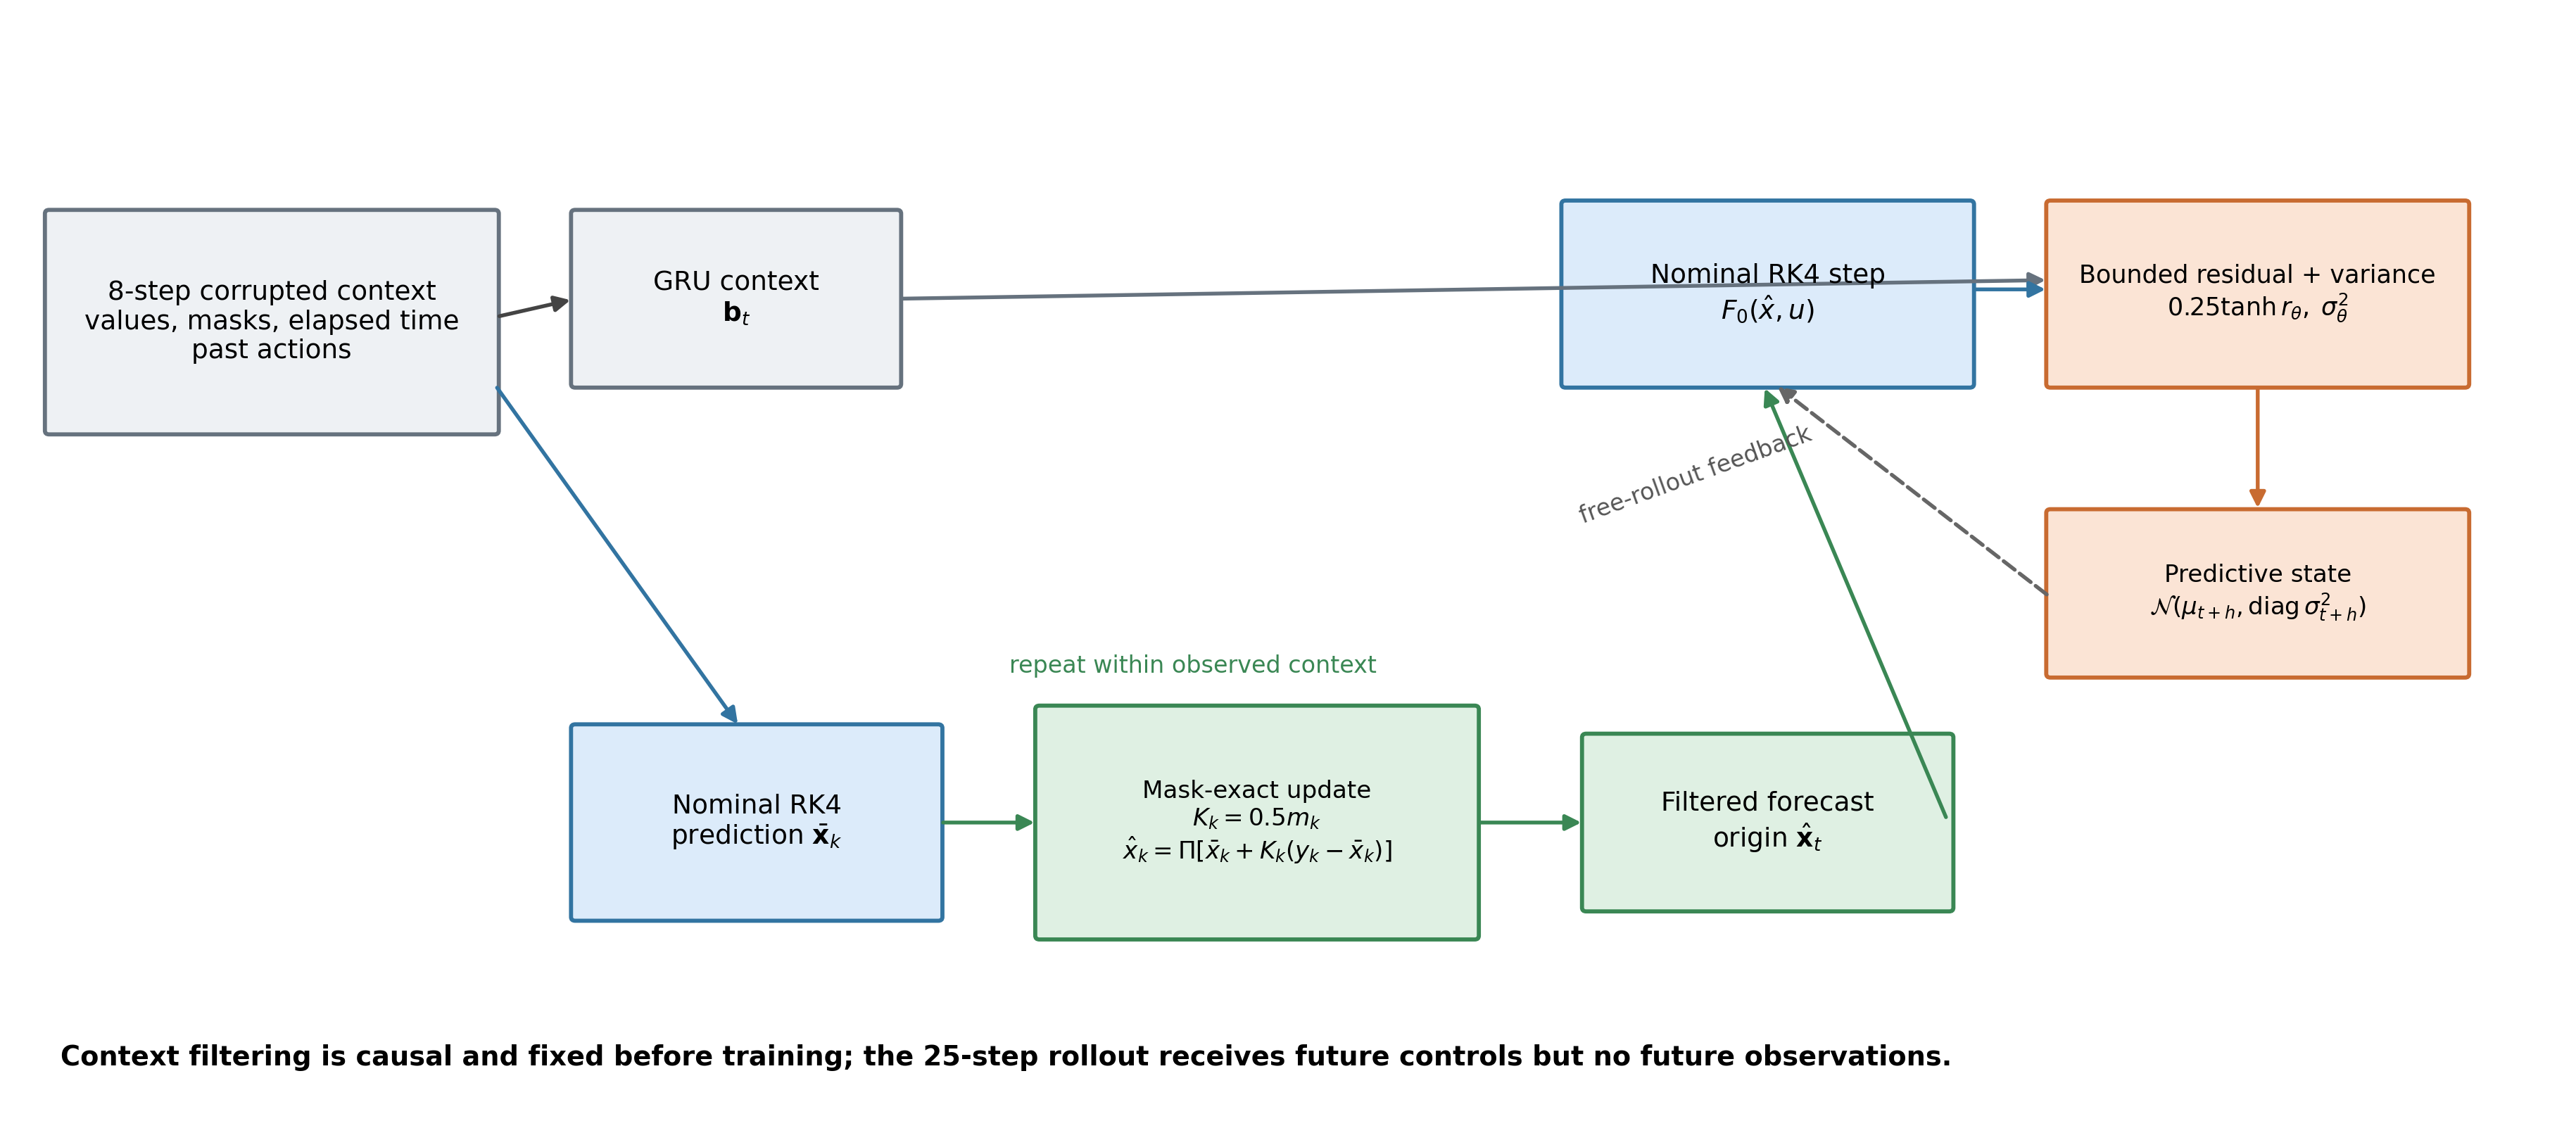
\includegraphics[width=0.96\textwidth]{figures/figure1_method.png}
\caption{Causal data flow of \method{}. A fixed complementary update is applied only inside the observed context. Missing channels receive exactly zero measurement gain. The filtered forecast origin then initializes a probabilistic nominal-physics plus neural-residual transition, which is rolled out freely for 25 steps using known future controls and no future observations.}
\label{fig:method}
\end{figure*}

\subsection{Forecasting problem}

Let $\vect{x}_t\in\mathbb{R}^{d_x}$ be a physical state and
$\vect{u}_t\in\mathbb{R}^{d_u}$ a recorded control. The observation available
to the model is
\begin{equation}
 \vect{y}_t=\vect{m}_t\odot(\vect{x}_t+\boldsymbol{\epsilon}_t),
\end{equation}
where $\vect{m}_t\in\{0,1\}^{d_x}$ is a channel-wise availability mask and
$\boldsymbol{\epsilon}_t$ is observation noise. Missing entries are filled
causally by the latest available value, producing $\tilde{\vect{y}}_t$; the
mask and elapsed time since observation $\boldsymbol{\delta}_t$ remain explicit
inputs to distinguish imputed values from fresh measurements.

At forecast origin $t$, the model receives eight context states and their past
controls,
\begin{equation}
 \mathcal C_t=\{\tilde{\vect y}_{t-7:t},\vect m_{t-7:t},
 \boldsymbol\delta_{t-7:t},\vect u_{t-7:t-1}\},
\end{equation}
together with known future controls $\vect u_{t:t+H-1}$. It estimates a
diagonal predictive distribution for $\vect{x}_{t+1:t+H}$ under free rollout,
with training horizon $H=25$, using predicted states at subsequent rollout
steps. The flight evaluation additionally extends rollout to $H=50$. All learned
operations use affine statistics estimated from the training split; the
nominal equations are evaluated in physical coordinates and then returned to
normalized coordinates.

\subsection{Mask-exact complementary context filter}

Let $F_0$ denote a nominal dynamics step: fourth-order Runge--Kutta integration
for the controlled benchmark, and the reduced flight model in
Section~\ref{sec:external}. Starting from the first imputed context vector, the
filter alternates nominal prediction and measurement update. For context index
$k>t-7$,
\begin{align}
 \bar{\vect x}_{k} &= F_0(\hat{\vect x}_{k-1},\vect u_{k-1}),\\
 \vect K_k &= \alpha\vect m_k,\qquad \alpha=0.5,\\
 \hat{\vect x}_k &= \Pi\!\left[
 \bar{\vect x}_k+\vect K_k\odot
 (\tilde{\vect y}_k-\bar{\vect x}_k)\right].
 \label{eq:complementary-update}
\end{align}
Thus, before projection, an observed channel receives equal weight from the
nominal prediction and the current measurement, while a missing channel has
exactly zero measurement correction. The projection $\Pi$ is the identity
except for the sine--cosine pendulum representation, which is returned to the
unit circle after each update. This joint projection couples the pendulum
channels and can change a channel whose measurement gain is zero. Mask-exactness
therefore describes the measurement correction before projection. The gain is
fixed before training, independently of validation and test outcomes.

In parallel, a GRU encodes
$[\tilde{\vect y}_k,\vect m_k,\log(1+\boldsymbol\delta_k),\vect u_{k-1}]$.
Its last hidden state supplies trajectory context to the forecast transition;
the measurement gain remains fixed. The implementation retains the
same unused gain-head parameterization in every controlled-benchmark
fixed-gain sensitivity model,
so comparisons at gains 0, 0.25, 0.5, 0.75, and 1 do not change nominal
capacity. This construction draws on filtering and data-assimilation approaches
\cite{revach2022_kalmannet,cheng2023_machine_learning_with_data_assimilation}
and uses the mask-exact context update to initialize a physics-residual
probabilistic world model.

\subsection{Probabilistic physics-residual rollout}

The last filtered context state initializes a free rollout. At step $h$,
\begin{align}
 \boldsymbol\mu^{p}_{t+h} &= F_0(\hat{\vect x}_{t+h-1},\vect u_{t+h-1}),\\
 [\vect r_{t+h},\vect \ell_{t+h}] &=
 R_\theta([\hat{\vect x}_{t+h-1},\vect u_{t+h-1},\vect b_{t+h-1}]),\\
 \boldsymbol\mu_{t+h} &= \Pi\!\left[
 \boldsymbol\mu^{p}_{t+h}+0.25\tanh(\vect r_{t+h})\right],\\
 \boldsymbol\sigma^2_{t+h} &=
 \max\!\left\{\exp\!\left(\operatorname{clip}(\vect\ell_{t+h},-8,4)\right),
 10^{-6}\right\}.
 \label{eq:residual-rollout}
\end{align}
The fixed residual scale bounds each normalized correction. The predicted mean
becomes the next state, and a GRUCell updates $\vect b$ from that mean and the
known control.

The training loss is the mean diagonal Gaussian negative log likelihood over
all $H$ steps and state channels,
\begin{equation}
 \mathcal L_{\mathrm{NLL}}=
 \frac{1}{2Hd_x}\sum_{h=1}^{H}\sum_{q=1}^{d_x}
 \left[\log(2\pi\sigma^2_{hq})+
 \frac{(x_{hq}-\mu_{hq})^2}{\sigma^2_{hq}}\right].
 \label{eq:nll}
\end{equation}
The one-step ablation applies the same loss only at $h=1$ but is still
evaluated by a 25-step free rollout.

\subsection{Causal execution and computational cost}

For each window, execution follows four deterministic stages. First, the GRU
encodes the imputed context together with masks, elapsed times, and past
controls. Second, Equation~\eqref{eq:complementary-update} advances the nominal
state through the same context and applies the mask-exact correction after each
available observation. Third, the final hidden state and filtered state jointly
initialize the residual recurrence. Fourth, Equation~\eqref{eq:residual-rollout}
is iterated for every known future control; predicted means, rather than samples
or targets, feed the next step. Training backpropagates the multi-step NLL
through this entire causal graph. Evaluation uses the identical graph with
gradients disabled, so teacher forcing is absent from both validation and test
rollouts.

Let $T_c$ denote context length, $H$ forecast horizon, $d_b$ recurrent width,
and $C_{F_0}$ the cost of one nominal step. Dense recurrent operations cost
$O((T_c+H)d_b^2)$ per trajectory, while nominal propagation costs
$O((T_c+H)C_{F_0})$. Diagonal mean and variance storage is $O(Hd_x)$; recurrent
working memory at inference is $O(d_b+d_x)$. Thus inference grows linearly in
context and horizon. The fixed filter adds nominal context steps; measured
latency captures their cost in the implementation.

\subsection{Forecast-origin and rollout error}

For an observed scalar channel on which $\Pi$ is the identity, write the
nominal pre-update error as $e_p=\bar x-x$ and measurement error as
$\epsilon=y-x$. Before any non-identity projection, Equation
\eqref{eq:complementary-update} gives the exact post-update error
\begin{equation}
 e_f=(1-\alpha)e_p+\alpha\epsilon.
\end{equation}
If these errors are zero-mean and uncorrelated, then
\begin{equation}
 \mathbb E[e_f^2]=(1-\alpha)^2\mathbb E[e_p^2]
 +\alpha^2\mathbb E[\epsilon^2].
 \label{eq:filter-mse}
\end{equation}
The benefit of equal trust depends on the relative sizes of the two error
terms. A missing channel has zero gain and therefore receives no direct
measurement-error term. For the pendulum's joint sine--cosine projection,
Equation~\eqref{eq:filter-mse} applies before projection; the projected error
also includes the coupled projection contribution. These dependencies motivate
the fixed-gain sensitivity analysis.

If the rollout transition is locally $L$-Lipschitz and incurs local error
$\eta_h$, the standard recursion yields
\begin{equation}
 \|\hat{\vect x}_{t+H}-\vect x_{t+H}\|
 \le L^H\|\hat{\vect x}_t-\vect x_t\|
 +\sum_{h=0}^{H-1}L^{H-1-h}\eta_h.
\end{equation}
The context filter acts on the initial-error term, while the residual model
must control subsequent local errors. The bound makes these two contributions
to long-horizon forecasting explicit.

\section{Controlled benchmark design}

\subsection{Controlled systems, corruption, and shift}

We evaluate five action-conditioned nonlinear systems. The damped oscillator
has state $(q,\dot q)$ and dynamics $m\ddot q+c\dot q+kq=u$; the Duffing
oscillator follows $\ddot q+c\dot q+\alpha q+\beta q^3=u$; and the controlled
Van der Pol system follows
$\ddot q=\mu(1-q^2)\dot q-q+g_u u$. The pendulum is represented by
$(\sin\theta,\cos\theta,\dot\theta)$, and the cart--pole by
$(x,\dot x,\theta,\dot\theta)$. Reference trajectories use fourth-order
Runge--Kutta integration with four internal substeps. Initial conditions,
bounded filtered stochastic controls, and physical parameters are generated
from recorded seeds. Shifted parameter intervals are prespecified and disjoint
from training intervals; unit tests verify that separation.

Each seed--system dataset contains 256 training, 64 validation, and 96 ID test
trajectories, plus 96 independently generated OOD test trajectories. A
trajectory has 72 states. Windows contain eight context states and 25 forecast
transitions; training and validation strides are eight and 16, respectively,
whereas evaluation uses one window per trajectory. Split identifiers encode
system, parameter regime, split, trajectory index, and generation seed. No
trajectory crosses splits.

The three evaluation regimes are (i) clean ID context, (ii) ID context with
feature-wise Gaussian noise at 8\% of the mean training-state standard
deviation and a nominal 25\% independent missing-at-random probability, and
(iii) the same corruption with OOD physical parameters. Training context uses
3\% noise and a nominal 10\% missing probability. The first time point of every
generated trajectory is forced observed in every channel so causal last-value
imputation is defined; masks at all subsequent trajectory time points are
sampled independently. A later sliding window can therefore begin at an
unobserved, causally imputed context value. Masks and channel-wise elapsed times
are retained. ID-clean and ID-corrupt evaluations reuse the same underlying 96
trajectories, permitting repeated-measurement resampling. OOD identifiers are
required to be disjoint from ID identifiers.

\subsection{Comparators, sensitivities, and candidate selection}

The five broad comparators cover recurrent, normalized, transformer, and
physics-guided transition families. \textbf{RSSM-style} is a compact recurrent
stochastic-style transition. \textbf{SimNorm-style} applies grouped simplex
normalization to its recurrent representation, adapting a representation
principle used by scalable continuous-control world models
\cite{hansen2023_td_mpc2_scalable_robust_world}. \textbf{Transformer-style} uses a
two-layer causal context transformer followed by recurrent free rollout
\cite{micheli2022_transformers_are_sample_efficient_world}. \textbf{PGNN-style}
adds a deterministic neural correction to a nominal physics step
\cite{robinson2022_physics_guided_neural_networks_for}. \textbf{PG-DMM-style} is a
probabilistic physics-residual transition inspired by physics-guided Deep
Markov modeling \cite{liu2022_physics_guided_deep_markov_models}. These are
protocol-matched transition implementations, not reproductions of published
end-to-end agents or their reported returns.

The proposed \textbf{\method} uses gain 0.5. Four fixed-gain sensitivities use
$\alpha\in\{0,0.25,0.75,1\}$, and \textbf{CFR-one-step} changes only the
training horizon. All six CFR variants have hidden width 72 and identical
parameterization; even the inactive fixed-gain head is retained. Comparator
widths are 80 for RSSM-style and SimNorm-style, 48 for Transformer-style, and
84 for PGNN-style and PG-DMM-style.

Candidate selection was separated from confirmation. A first development
model, reliability-gated RGP-WM, failed its corrected primary hypothesis after
an audit replaced a trajectory-local NRMSE denominator by a training-only
scale. A structurally distinct learned-gain PFR-WM then improved over the retrained
PGNN-style comparator on development seed 11, but exceeded its prespecified gain-0.5 matched
ablation by 0.223\%, below the frozen 2\% mechanism threshold. Learned
gain was therefore rejected and is absent from every confirmatory seed. The
gain-0.5 comparator from that failed mechanism test became the versioned
CFR-WM candidate before confirmation. Original development outputs, corrected
re-evaluations, and failure decisions remain archived; none is pooled with the
confirmatory analysis.

\subsection{Optimization and endpoint definitions}

All models use AdamW, batch size 128, gradient clipping at norm 5, at most 60
epochs, and early stopping after ten epochs without a validation-NLL
improvement of $10^{-5}$. The pre-confirmation tuning archive contains the same
six-trial validation budget for every baseline--system pair. Each baseline uses
its own frozen winner. CFR-WM and all CFR sensitivities inherit the frozen PGNN-style
winner for the same system. All hyperparameters were fixed before confirmation.

The primary endpoint is NRMSE through horizon 25. Per-feature RMSE is divided
by that feature's standard deviation estimated from the training split only,
then averaged over features. Because stored targets and predictions are already
in those normalized coordinates, the evaluation divisor is one. This avoids
estimating a denominator from the test trajectory and remains defined at
horizon one. Secondary accuracy endpoints are cumulative NRMSE at horizons 1,
5, and 10 and MAE through horizon 25. Probabilistic endpoints are diagonal
Gaussian NLL, empirical 90\% coverage, mean 90\% interval width, and mean
absolute central-interval calibration error over nominal levels 0.1--0.9. A
trajectory is catastrophic when any feature-step absolute error exceeds three
training-set standard deviations.

\subsection{Frozen confirmatory inference}

The confirmation grid contains 11 methods, eight untouched seeds
$(41,53,67,79,83,97,109,113)$, five systems, and three regimes: 440 training
runs, 1,320 aggregate cells, and 126,720 paired trajectory rows. One
deterministic dataset fingerprint is shared by all methods within each
seed--system group, and all 40 such fingerprints must be distinct. The eight
seed-level training/data realizations are the top-level independent clusters;
trajectories are nested observations. Inference conditions on the fixed set of
systems and regimes.

For a seed $s$, let $B_s$ and $C_s$ be the PGNN-style and CFR-WM NRMSE-25 means after
equal weighting of all 15 system--regime cells. The primary estimand is
\begin{equation}
 \Delta_{\mathrm{rel}}=\frac{1}{8}\sum_{s=1}^{8}
 100\frac{B_s-C_s}{B_s}.
 \label{eq:primary-estimand}
\end{equation}
A 5,000-replicate bootstrap resamples seeds globally with replacement. Within
each selected seed and system it resamples paired trajectory identifiers;
ID-clean and ID-corrupt reuse the same sampled identifier vector, while the
disjoint OOD set is resampled independently. Every system--regime cell is
retained, and $B_s$, $C_s$, and their ratio are recomputed in each replicate.
The interval is the two-sided percentile 95\% interval.

H1 states that \method{} improves on the preselected PGNN-style comparator by at least 5\%.
Support requires finite metrics, a lower relative-improvement interval endpoint
of at least 5\%, and a one-sided exact sign-flip $p<0.05$ for the seed effects
after subtracting the 5\% margin. All $2^8$ sign configurations are enumerated
under a prespecified symmetry assumption. Confirmation success is determined
by H1 alone.

H2 is tested only if H1 succeeds. It requires at least 5\% improvement when
pooling ID-corrupt and OOD-corrupt fixed cells, and clean-regime
noninferiority with signed relative-improvement margin $-5\%$. Both components
must meet their respective bootstrap bound and one-sided margin test, with all
metrics finite. The five broad CFR-versus-comparator contrasts form one Holm
family; the five CFR sensitivity/ablation contrasts form another. With eight
clusters, the minimum two-sided exact raw and five-test Holm-adjusted values are
$2/2^8=0.0078125$ and 0.0390625. The 15 system--regime contrasts report paired
effects and unadjusted bootstrap intervals as descriptive estimates.

\subsection{Reproducibility controls}

The frozen contract fixes code hashes, configurations, data identities,
trajectory pairing, and finite-metric checks. A metadata-loader amendment was
frozen before performance inspection and left inferential functions and decision
rules unchanged. Full provenance, amendment details, and recovery controls
appear in the appendix.

Execution uses Python 3.11.15 and PyTorch 2.11.0+cu130 on an NVIDIA RTX 5070
Laptop GPU with 8,151 MiB reported memory and an AMD Ryzen 9 9955HX processor.
The sequential runner stops at 80\% of an eight-hour budget and writes each
condition atomically.

\section{Controlled benchmark results}

\subsection{Aggregate accuracy}

The confirmatory analyzer accepted the complete grid of \ConfirmatoryRuns{}
trained models and \ConfirmatoryTrajectories{} trajectory-level rows. All
prespecified metrics were finite (\AllMetricsFinite), and the 40 seed--system
groups produced \UniqueDataHashes{} distinct data fingerprints while sharing
one fingerprint across methods within each group, confirming grid completeness
and pairing.

Table~\ref{tab:main-results} reports the seed-balanced mean and standard
deviation for horizons 1, 10, and 25. Across all 11 methods, \BestMethod{}
had the lowest aggregate NRMSE-25 (\BestNRMSE). CFR-WM's mean was
\CFRNRMSE{}, compared with \PGNNNRMSE{} for the preselected PGNN-style comparator.

\begin{table*}[t]
\centering
\caption{Confirmatory accuracy over the fixed five-system, three-regime
benchmark. Entries are means $\pm$ SD across eight seed-level, cell-balanced
aggregates. Bold marks the lowest aggregate NRMSE-25. Parameter counts are means
over the five system-specific input dimensions; all methods received the same six-trial
validation search budget.}
\label{tab:main-results}
\resizebox{\textwidth}{!}{\begin{tabular}{lrrrr}
\toprule
Method & Mean parameters & NRMSE-1 & NRMSE-10 & NRMSE-25 \\
\midrule
CFR-WM & 57694 & 0.039 $\pm$ 0.001 & 0.057 $\pm$ 0.002 & \textbf{0.100 $\pm$ 0.004} \\
CFR-gain-0.25 & 57694 & 0.037 $\pm$ 0.001 & 0.059 $\pm$ 0.002 & 0.103 $\pm$ 0.004 \\
CFR-gain-0.75 & 57694 & 0.047 $\pm$ 0.001 & 0.065 $\pm$ 0.002 & 0.107 $\pm$ 0.005 \\
PGNN-style & 61275 & 0.060 $\pm$ 0.001 & 0.070 $\pm$ 0.002 & 0.110 $\pm$ 0.003 \\
CFR-gain-1 & 57694 & 0.059 $\pm$ 0.001 & 0.073 $\pm$ 0.002 & 0.114 $\pm$ 0.004 \\
PG-DMM-style & 61493 & 0.063 $\pm$ 0.001 & 0.075 $\pm$ 0.002 & 0.114 $\pm$ 0.003 \\
RSSM-style & 62485 & 0.073 $\pm$ 0.002 & 0.090 $\pm$ 0.005 & 0.123 $\pm$ 0.006 \\
Transformer-style & 59708 & 0.074 $\pm$ 0.002 & 0.094 $\pm$ 0.004 & 0.132 $\pm$ 0.009 \\
SimNorm-style & 62485 & 0.074 $\pm$ 0.002 & 0.098 $\pm$ 0.006 & 0.138 $\pm$ 0.013 \\
CFR-gain-0 & 57694 & 0.081 $\pm$ 0.003 & 0.100 $\pm$ 0.003 & 0.144 $\pm$ 0.005 \\
CFR-one-step & 57694 & 0.040 $\pm$ 0.001 & 0.136 $\pm$ 0.050 & 0.278 $\pm$ 0.104 \\
\bottomrule
\end{tabular}
}
\end{table*}

\begin{quote}
\small\textbf{Frozen primary estimand.} For each seed, PGNN-style and CFR-WM
NRMSE-25 are first averaged with equal weight over the 15 prespecified
system--regime cells; their relative improvement is then computed. The
confirmatory point estimate is the arithmetic mean of those eight seed-level
relative improvements, not the ratio of the two pooled means in
Table~\ref{tab:main-results}.
\end{quote}

\subsection{Primary and gated robustness hypotheses}

Against PGNN-style, the seed-mean relative NRMSE-25 improvement was
\PrimaryImprovement\% (95\% paired fixed-cell bootstrap CI
[\PrimaryRelativeCILow\%, \PrimaryRelativeCIHigh\%]). In absolute units,
CFR-WM minus PGNN-style was \PrimaryDifference{} (95\% CI [\PrimaryCILow,
\PrimaryCIHigh]). The exact one-sided sign-flip test against the same 5\%
practical margin gave $p=\PrimaryPValue$. Under the frozen conjunction of a
5\% interval lower bound, $p<0.05$, and finite metrics, H1 was
\PrimaryDecision.

For the H2 components, the combined corrupt-ID and corrupt-OOD regimes had a
relative effect of \CorruptImprovement\% (95\% CI
[\CorruptRelativeCILow\%, \CorruptRelativeCIHigh\%], one-sided 5\%-margin
$p=\CorruptPValue$). ID-clean had an effect of \CleanImprovement\% (95\% CI
[\CleanRelativeCILow\%, \CleanRelativeCIHigh\%], one-sided signed
$-5\%$-margin $p=\CleanPValue$). Because H2 is hierarchically gated by H1 and
requires both component rules, the robustness hypothesis was
\RobustnessDecision.

Table~\ref{tab:seed-effects} reports the eight independent cluster effects.
Every seed exceeded the 5\% practical threshold.

\begin{table}[t]
\centering
\caption{Seed-level primary effects after equal weighting of the 15 frozen
benchmark cells. Positive values favor CFR-WM.}
\label{tab:seed-effects}
\begin{tabular}{rr}
\toprule
Seed & CFR-WM improvement over PGNN-style, \% \\
\midrule
41 & +5.29 \\
53 & +12.76 \\
67 & +12.01 \\
79 & +10.49 \\
83 & +9.69 \\
97 & +6.66 \\
109 & +9.32 \\
113 & +5.56 \\
\bottomrule
\end{tabular}

\end{table}

\begin{figure*}[t]
\centering
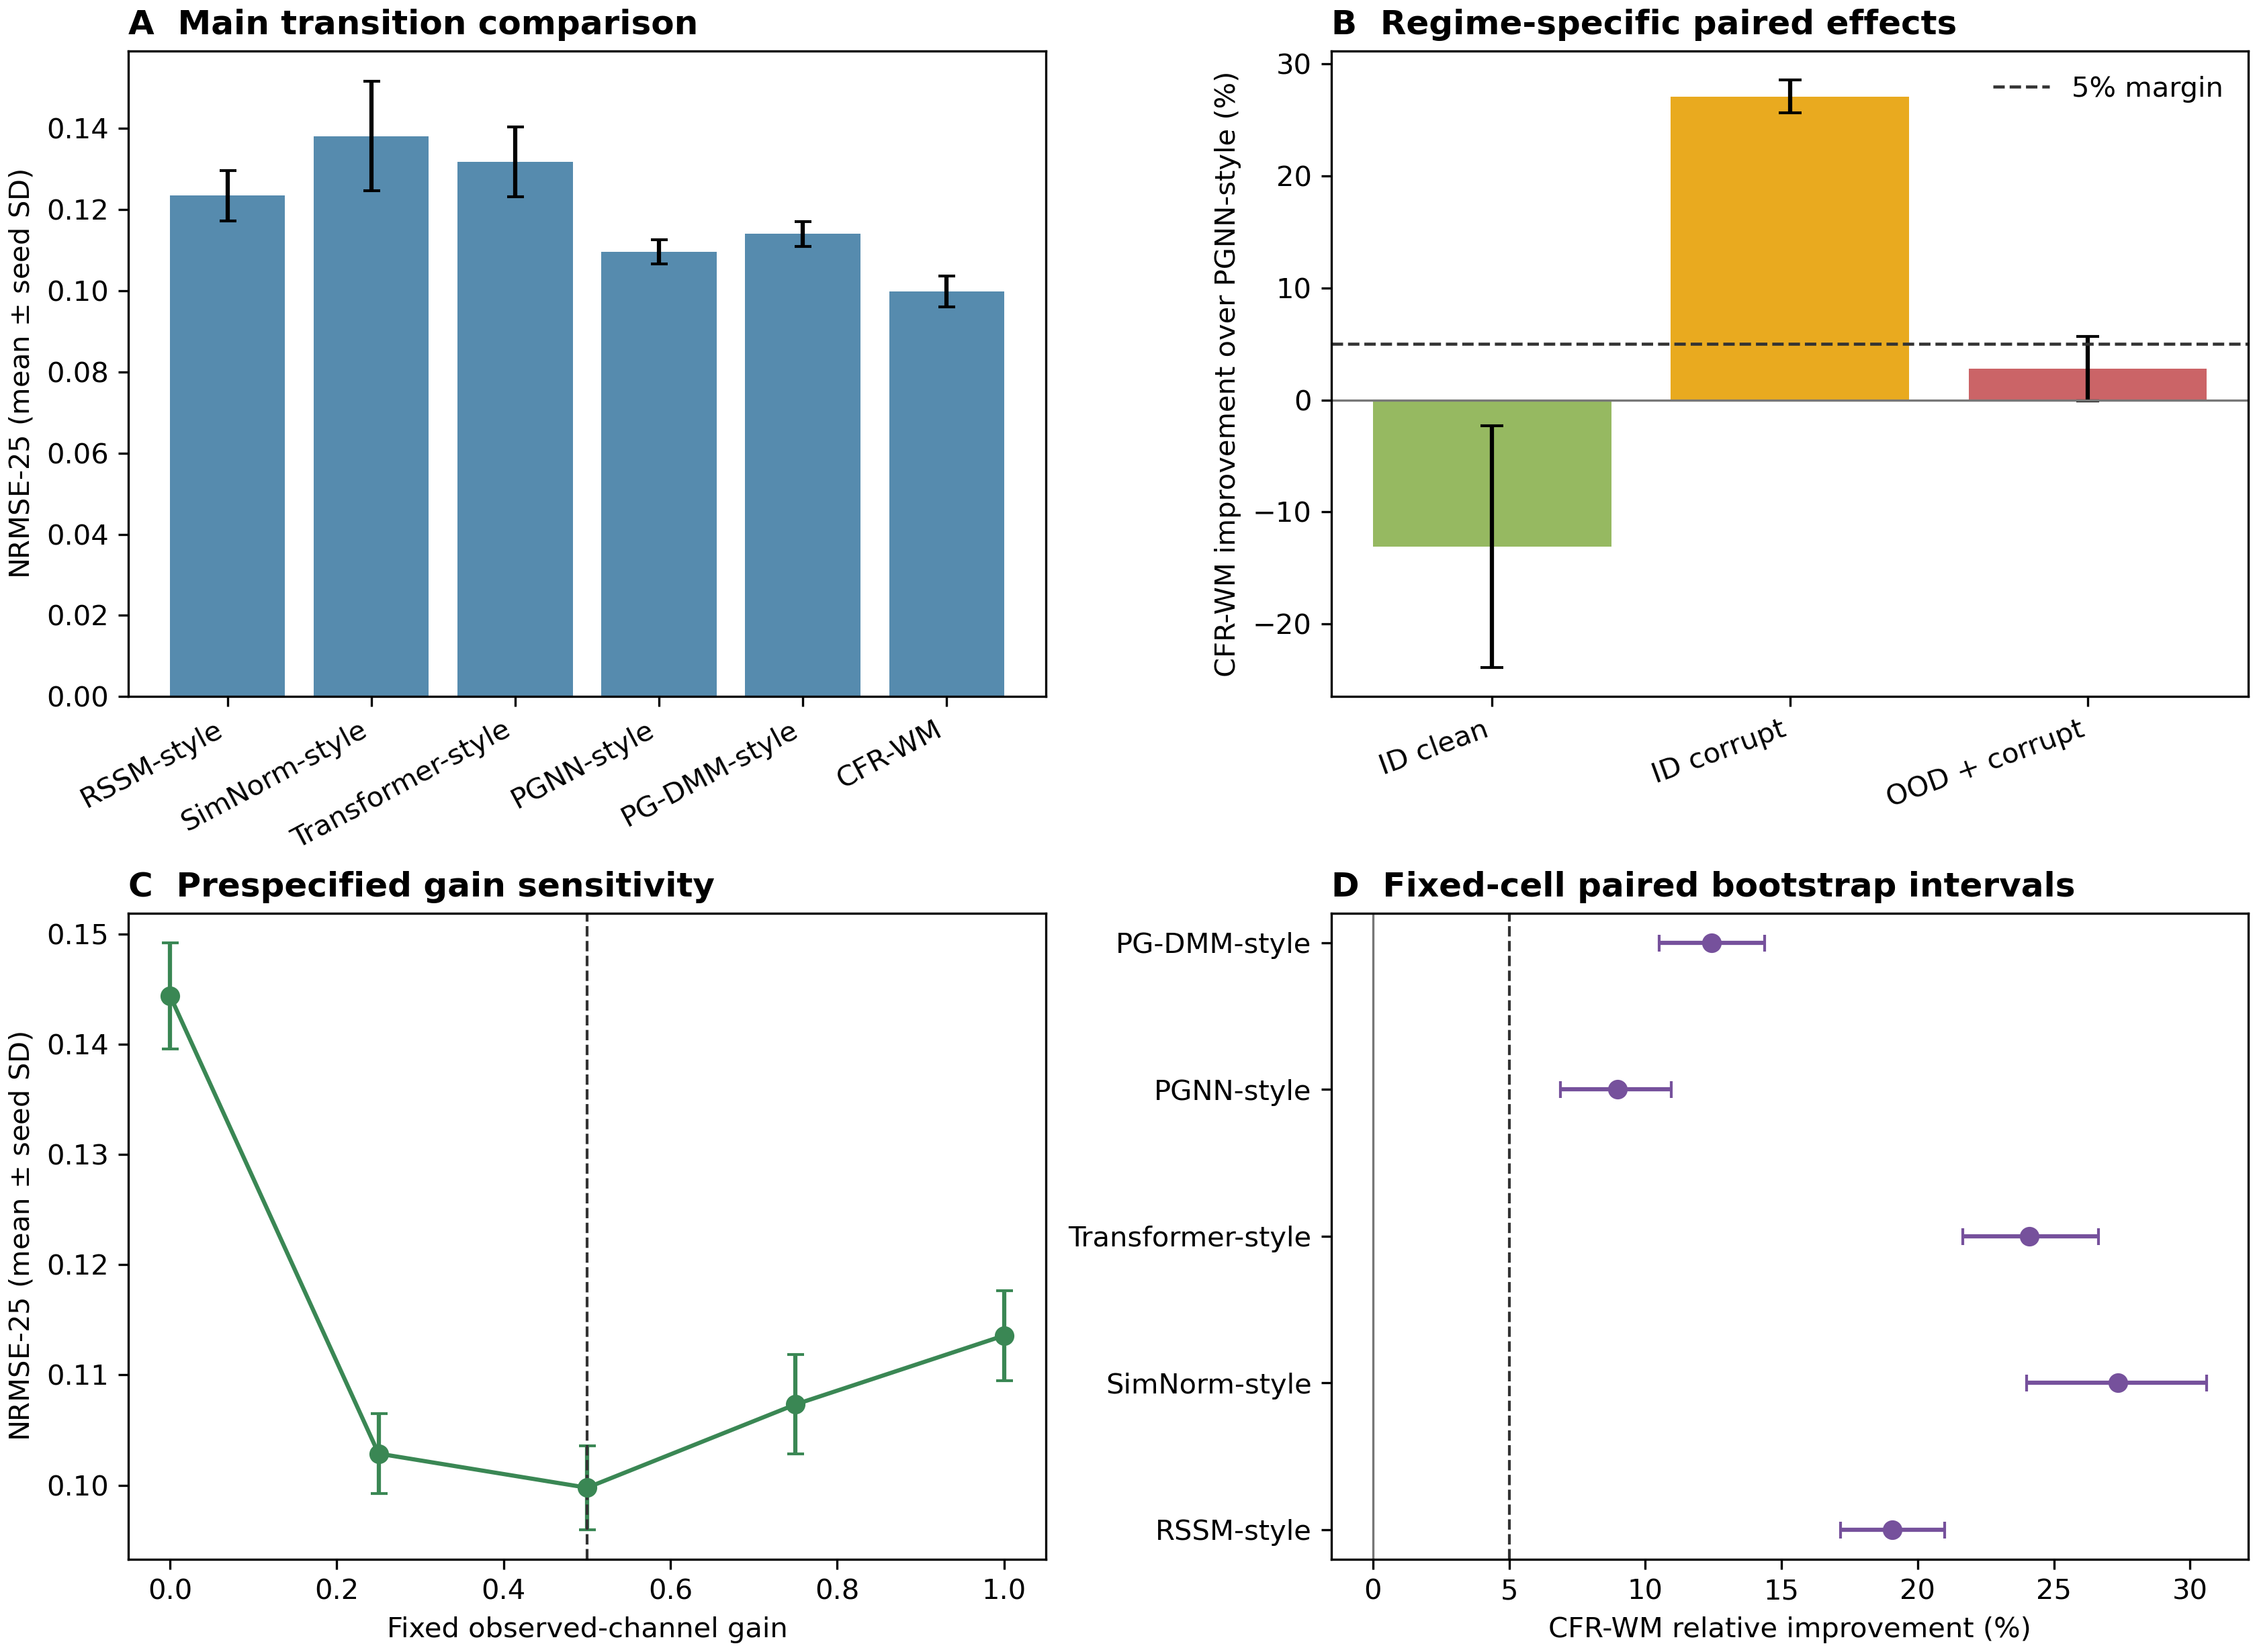
\includegraphics[width=0.96\textwidth]{figures/confirmatory_overview.png}
\caption{Locked confirmatory summary. (A) Aggregate transition accuracy for the
six main methods. (B) Paired CFR-WM effects against PGNN-style by regime; positive
values favor CFR-WM. (C) Prespecified fixed-gain sensitivity. (D) Paired
fixed-cell intervals against each broad comparator. Error bars in A--C are
seed-level SD; D uses the nested 95\% bootstrap interval.}
\label{fig:confirmatory-overview}
\end{figure*}

\subsection{Comparator and sensitivity evidence}

Table~\ref{tab:comparator-contrasts} reports every prespecified broad
comparison. Positive relative effects favor CFR-WM. The confidence intervals
retain all fixed cells, whereas the exact two-sided seed sign-flip values are
Holm-adjusted as one five-test family. These secondary comparisons contextualize
the primary PGNN-style contrast.

The PGNN-style row repeats the primary point estimate but uses the frozen
comparator-family bootstrap seed (20260808), whereas H1 uses its prespecified
primary seed (20260805). The estimand and 5,000-replicate resampling scheme are
otherwise identical; the separately sampled interval endpoints differ by at
most 0.01 percentage point after rounding, and only the primary interval enters
the H1 decision.

\begin{table*}[t]
\centering
\caption{CFR-WM relative NRMSE-25 effects against broad comparators. Exact
$p$ values test a zero seed-level difference; Holm adjustment is confined to
this prespecified family of five.}
\label{tab:comparator-contrasts}
\begin{tabular}{lrrr}
\toprule
Reference & Relative effect [95\% CI], \% & Exact $p$ & Holm $p$ \\
\midrule
RSSM-style & +19.08 [+17.16, +20.98] & 0.0078 & 0.0391 \\
SimNorm-style & +27.34 [+24.00, +30.62] & 0.0078 & 0.0391 \\
Transformer-style & +24.09 [+21.65, +26.64] & 0.0078 & 0.0391 \\
PGNN-style & +8.97 [+6.89, +10.96] & 0.0078 & 0.0391 \\
PG-DMM-style & +12.44 [+10.51, +14.39] & 0.0078 & 0.0391 \\
\bottomrule
\end{tabular}

\end{table*}

The lowest aggregate NRMSE-25 among gains $0$, $0.25$, $0.5$, $0.75$, and $1$
occurred at gain \BestGain. Relative to the one-step-trained variant, CFR-WM's
effect was \OneStepImprovement\% (95\% CI [\OneStepRelativeCILow\%,
\OneStepRelativeCIHigh\%], Holm $p=\OneStepHolmP$). Table
\ref{tab:sensitivity-contrasts} gives the complete second five-test family.

\begin{table*}[t]
\centering
\caption{CFR-WM relative NRMSE-25 effects against gain and training-horizon
sensitivities. Positive values favor the proposed gain-0.5 multi-step model.}
\label{tab:sensitivity-contrasts}
\begin{tabular}{lrrr}
\toprule
Reference & Relative effect [95\% CI], \% & Exact $p$ & Holm $p$ \\
\midrule
Gain 0 & +30.89 [+28.95, +32.67] & 0.0078 & 0.0391 \\
Gain 0.25 & +2.97 [+0.88, +5.27] & 0.0312 & 0.0391 \\
Gain 0.75 & +6.97 [+4.77, +9.42] & 0.0078 & 0.0391 \\
Gain 1 & +12.13 [+10.31, +13.92] & 0.0078 & 0.0391 \\
One-step training & +59.38 [+48.88, +68.88] & 0.0078 & 0.0391 \\
\bottomrule
\end{tabular}

\end{table*}

Table~\ref{tab:secondary} reports secondary diagnostics of Gaussian forecast
quality, marginal calibration, and catastrophic-rollout frequency.

\begin{table*}[t]
\centering
\caption{Secondary aggregate diagnostics for the six broad methods. Rates and
scores are seed-balanced over all fixed cells and are not separately tested.}
\label{tab:secondary}
\resizebox{\textwidth}{!}{\begin{tabular}{lrrrr}
\toprule
Method & Parameters & Gaussian NLL & Calibration error & Catastrophic rate \\
\midrule
RSSM-style & 62485 & -0.183 & 0.214 & 0.01\% \\
SimNorm-style & 62485 & -0.246 & 0.206 & 0.01\% \\
Transformer-style & 59708 & -0.279 & 0.202 & 0.01\% \\
PGNN-style & 61275 & -0.385 & 0.248 & 0.00\% \\
PG-DMM-style & 61493 & 0.029 & 0.245 & 0.00\% \\
CFR-WM & 57694 & 0.013 & 0.228 & 0.00\% \\
\bottomrule
\end{tabular}
}
\end{table*}

\subsection{Fixed-cell heterogeneity}

Figure~\ref{fig:cell-heterogeneity} retains all 15 system--regime effects. By
the frozen descriptive guard, CFR-WM was more than 10\% worse than PGNN-style in
\CellsWorseTen{} cells. All three were ID-clean: cart--pole
(\CartpoleCleanChange\% relative change), controlled Van der Pol
(\VanDerPolCleanChange\%), and Duffing (\DuffingCleanChange\%). Conversely,
\IDCorruptFavoredCount{} of \IDCorruptCellCount{} ID-corrupt cells favored
CFR-WM, with descriptive changes from \IDCorruptLeastChange\% to
\IDCorruptMostChange\%. This pattern explains why an aggregate H1 success coexists with
failure of clean-regime noninferiority. These cell-level estimates are
descriptive; their unadjusted bootstrap intervals are reported in the appendix
table and machine-readable CSV.

\begin{figure}[t]
\centering
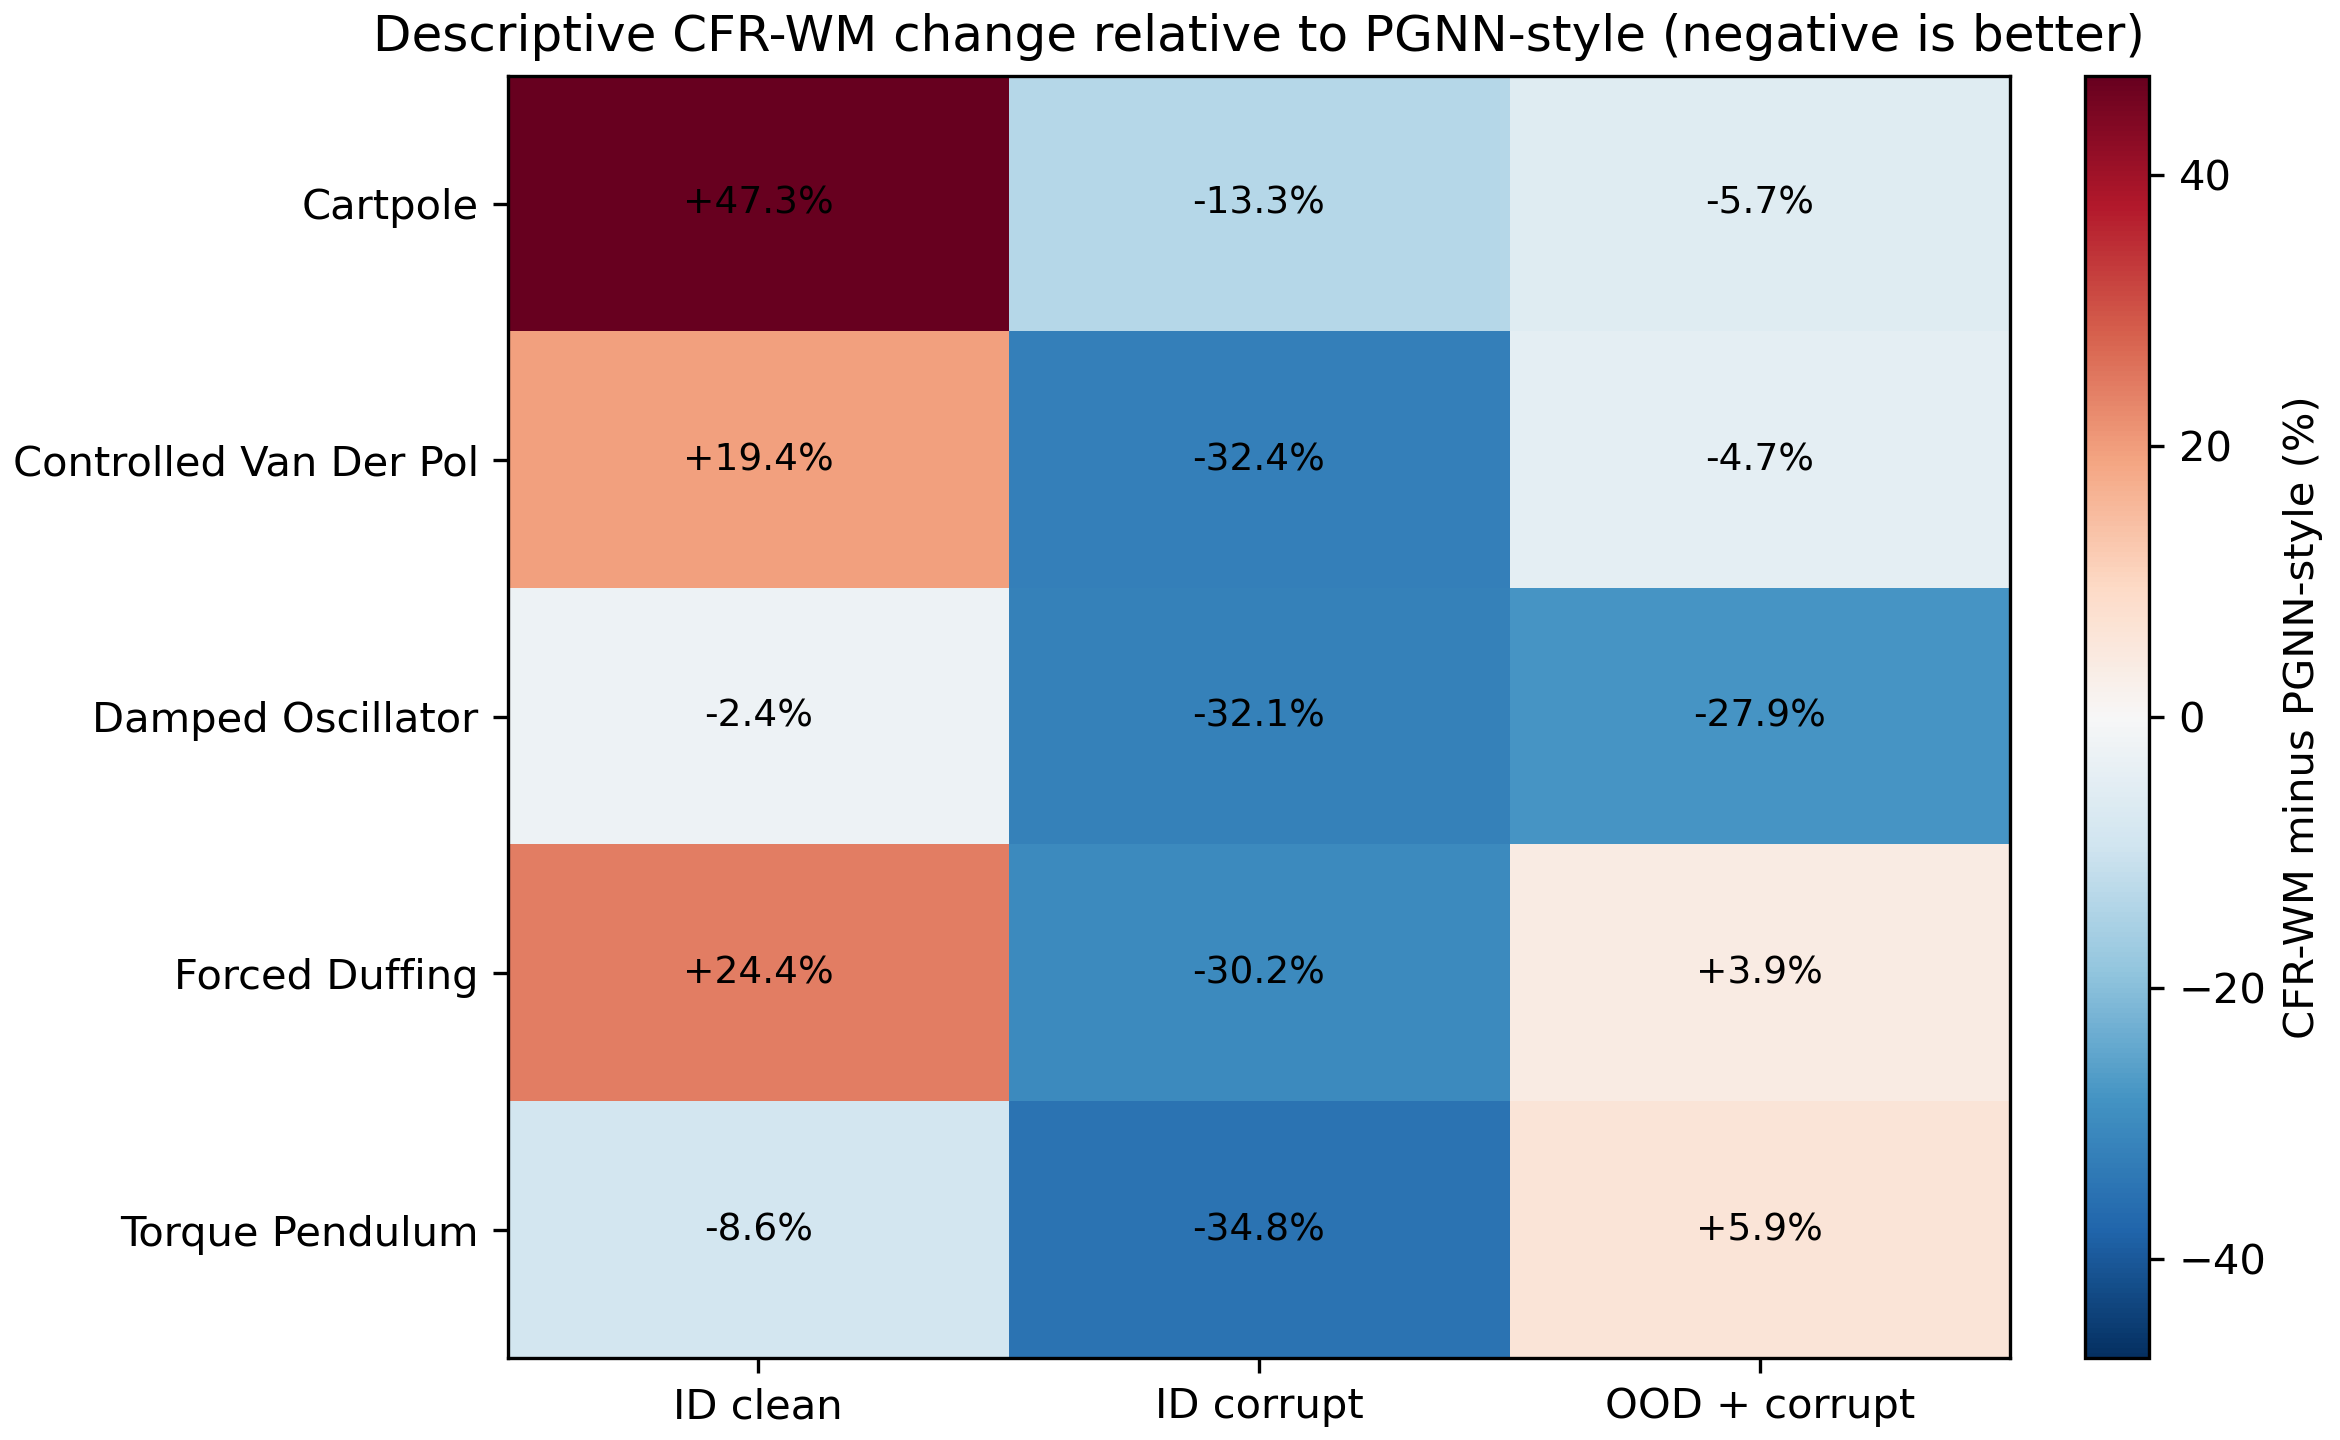
\includegraphics[width=\linewidth]{figures/cell_difference_heatmap.png}
\caption{Descriptive CFR-WM change relative to PGNN-style in each fixed benchmark
cell. Negative values mean lower NRMSE-25 for CFR-WM.}
\label{fig:cell-heterogeneity}
\end{figure}

\section{External evaluation on measured drone flights}
\label{sec:external}

\subsection{Data, held-out trajectories, and physical prior}

We extend the controlled study to the NanoDrone benchmark, which records
Crazyflie 2.1 Brushless flights using motion capture and onboard sensors
\cite{busetto2026_nanodrone}. The released records include the authors'
offline synchronization, 100\,Hz resampling, motor--acceleration alignment,
and zero-phase low-pass filtering. We retain these records and predict their
recorded state estimates. Position, velocity, rotation-vector orientation,
and body angular velocity form a 12-coordinate state; four motor angular
speeds are the inputs.

Complete flights define the split. Runs 1--3 of Square, Random, and Chirp
provide nine training records (41,700 samples); run 4 of each supplies three
validation records (13,899 samples). Three Melon flights (19,497 samples)
test a trajectory family absent from training. This validation holdout is an
addition to the authors' training/test partition. Windows remain within
flights, and normalization uses training samples only.

The nominal model combines gravity with thrust along the body vertical axis:
\begin{equation}
 a_t=c_T R(r_t)e_3\sum_{j=1}^{4}\omega_{j,t}^{2}-g e_3,
 \qquad
 v_{t+1}=v_t+\Delta t\,a_t,\quad
 p_{t+1}=p_t+\Delta t\,v_t+\tfrac12\Delta t^2a_t.
 \label{eq:flight-prior}
\end{equation}
Here $r_t$ is the rotation vector, $\omega_{j,t}$ is motor speed,
$g=9.81\,\mathrm{m\,s^{-2}}$, and $\Delta t=0.01$\,s. A nonnegative
least-squares fit on training transitions gives
$c_T=8.31887655\times10^{-7}$ in
$(\mathrm{m\,s^{-2}})/(\mathrm{rad\,s^{-1}})^2$.
Orientation advances by quaternion composition under constant body angular
velocity. The prior omits angular acceleration, drag, and motor lag, adding
structural mismatch to the parameter mismatch studied in the simulations.

\subsection{Matched comparisons and evaluation protocol}

The flight implementation uses a width-64 recurrent encoder and residual
transition. Three learned models share \ExternalLearnedParameters{} parameters:
CFR-WM with gain 0.5, an unfiltered physics-residual model, and a data-only
recurrent transition. The latter replaces the nominal physics step with a
learned increment; the unfiltered model starts from the final imputed
measurement. All three use the same encoder, bounded correction, and
diagonal-Gaussian likelihood. The context GRU receives 40 features; a
width-64 GRU cell advances the hidden state from 12 predicted coordinates and
four inputs. An $80\!\to\!64\!\to\!64\!\to\!24$ SiLU head outputs
12 corrections and 12 log variances. Corrections use $0.25\tanh(\cdot)$ in
normalized coordinates, and log variances are clipped to $[-8,4]$.
A nominal-only forecast supplies a fourth
reference. These matched implementations follow the physics, hybrid, and
recurrent families represented in the NanoDrone benchmark.

Each window contains eight context states. Last-value imputation and elapsed
missingness times are computed within each flight before window extraction,
so an imputed entry can retain an observation preceding the eight-state
context. Training uses an equal mixture of recorded contexts and contexts
with Gaussian noise of 0.05 training standard deviations per coordinate and
10\% independent missingness. Controls and targets are unchanged. All learned
models train on 25-step rollouts with stride 10, AdamW, batch size 256, at most
40 epochs, and eight-epoch early stopping. Each method selects between
learning rates 0.001 and 0.003 by validation NLL using development seed 17,
then trains with five final seeds (131, 149, 167, 181, 199).

Evaluation uses four paired context conditions: as recorded, Gaussian noise
only (0.1 training standard deviations), missingness only (30\%), and their
combination. The same perturbation realization is shared across methods and
training seeds. Known recorded motor inputs drive free forecasts through
25 and 50 steps (0.25 and 0.5\,s), with test stride 50. For flight $f$, model
$m$, and horizon $H$, the external score is
\begin{equation}
 E_{m,f,H}=\sqrt{\frac{1}{12H N_f}
 \sum_{i=1}^{N_f}\sum_{h=1}^{H}\sum_{d=1}^{12}
 \left(\frac{\widehat{x}_{m,i,h,d}-x_{i,h,d}}{s_d}\right)^2},
 \label{eq:external-score}
\end{equation}
where $s_d$ is the training standard deviation. This score takes one root
after pooling normalized squared errors; the controlled study instead
averages feature-wise normalized RMSE. External summaries first give the
three flights equal weight, then report the mean and sample SD across five
training seeds. Position and velocity scores use root-mean-square Euclidean
error in physical units. Paired relative improvements are averaged across
seeds after the same flight weighting.

The flight protocol was recorded before external test evaluation and executed
after the synthetic confirmation. Its descriptive comparisons extend the
empirical setting while retaining the original H1 and H2 decisions.

\subsection{Flight forecasting results}

Table~\ref{tab:external-results} reports all eight condition--horizon
comparisons. Each learned model has lower mean full-state NRMSE than the
nominal forecast. The unfiltered residual model has lower mean full-state
NRMSE than CFR-WM in all eight comparisons. With recorded contexts at 50 steps,
their scores are \ExternalUnfilteredRecordedLongNRMSEMean{} and
\ExternalCFRRecordedLongNRMSEMean{}, respectively. Combined noise and
missingness narrows this difference to
\ExternalUnfilteredCombinedLongNRMSEMean{} versus
\ExternalCFRCombinedLongNRMSEMean{}.
CFR-WM improves over the data-only recurrent model at 25 steps under added
noise and combined corruption, but its mean error is higher at 50 steps
in all four conditions.

The physical-unit scores distinguish position and velocity behavior
(Table~\ref{tab:external-physical}; Figure~\ref{fig:external-flight}).
CFR-WM has the lowest 50-step position error among the three learned models
in all four conditions. Under combined corruption, its position error is
\ExternalCFRCombinedLongPositionMean{}\,m, compared with
\ExternalUnfilteredCombinedLongPositionMean{}\,m for the unfiltered model.
The nominal prior has lower position error than the learned models on
recorded and missing-only contexts, despite its higher full-state error.
Velocity errors show a different ordering: CFR-WM is worse than the
unfiltered model on recorded and missing-only contexts, and nearly tied
under noise and combined corruption. Thus, the position benefit coexists
with a full-state accuracy cost on these held-out flights.

\begin{table*}[t]
\centering
\caption{External flight NRMSE (Equation~\ref{eq:external-score}). Entries
are means $\pm$ SD across five training seeds after equal weighting of three
held-out flights. The nominal forecast is deterministic. All four context
conditions and both horizons are retained.}
\label{tab:external-results}
\resizebox{\textwidth}{!}{\begin{tabular}{llrrrr}
\toprule
Context & Horizon & CFR-WM & Unfiltered & Recurrent & Nominal \\
\midrule
As recorded & 25 & $0.389 \pm 0.012$ & $0.376 \pm 0.010$ & $0.388 \pm 0.008$ & $0.488$ \\
As recorded & 50 & $0.530 \pm 0.016$ & $0.518 \pm 0.019$ & $0.519 \pm 0.006$ & $0.790$ \\
Noise & 25 & $0.393 \pm 0.012$ & $0.387 \pm 0.010$ & $0.398 \pm 0.008$ & $0.498$ \\
Noise & 50 & $0.532 \pm 0.017$ & $0.523 \pm 0.018$ & $0.527 \pm 0.006$ & $0.797$ \\
Missing & 25 & $0.397 \pm 0.011$ & $0.386 \pm 0.008$ & $0.395 \pm 0.005$ & $0.495$ \\
Missing & 50 & $0.537 \pm 0.014$ & $0.527 \pm 0.020$ & $0.526 \pm 0.007$ & $0.792$ \\
Noise + missing & 25 & $0.401 \pm 0.011$ & $0.397 \pm 0.008$ & $0.405 \pm 0.005$ & $0.506$ \\
Noise + missing & 50 & $0.540 \pm 0.014$ & $0.534 \pm 0.019$ & $0.533 \pm 0.006$ & $0.799$ \\
\bottomrule
\end{tabular}
}
\end{table*}

\begin{table*}[t]
\centering
\caption{External 50-step position and velocity error in physical units,
using the same flight and seed weighting as Table~\ref{tab:external-results}.}
\label{tab:external-physical}
\resizebox{\textwidth}{!}{\begin{tabular}{lrrrr}
\toprule
& \multicolumn{2}{c}{Position RMSE (m)} & \multicolumn{2}{c}{Velocity RMSE (m/s)} \\
Context & CFR-WM & Unfiltered & CFR-WM & Unfiltered \\
\midrule
As recorded & $0.078 \pm 0.003$ & $0.083 \pm 0.010$ & $0.249 \pm 0.015$ & $0.233 \pm 0.009$ \\
Noise & $0.091 \pm 0.003$ & $0.115 \pm 0.007$ & $0.257 \pm 0.014$ & $0.258 \pm 0.007$ \\
Missing & $0.081 \pm 0.005$ & $0.095 \pm 0.022$ & $0.259 \pm 0.014$ & $0.243 \pm 0.009$ \\
Noise + missing & $0.094 \pm 0.004$ & $0.125 \pm 0.017$ & $0.267 \pm 0.014$ & $0.268 \pm 0.009$ \\
\bottomrule
\end{tabular}
}
\end{table*}

\begin{figure*}[t]
\centering
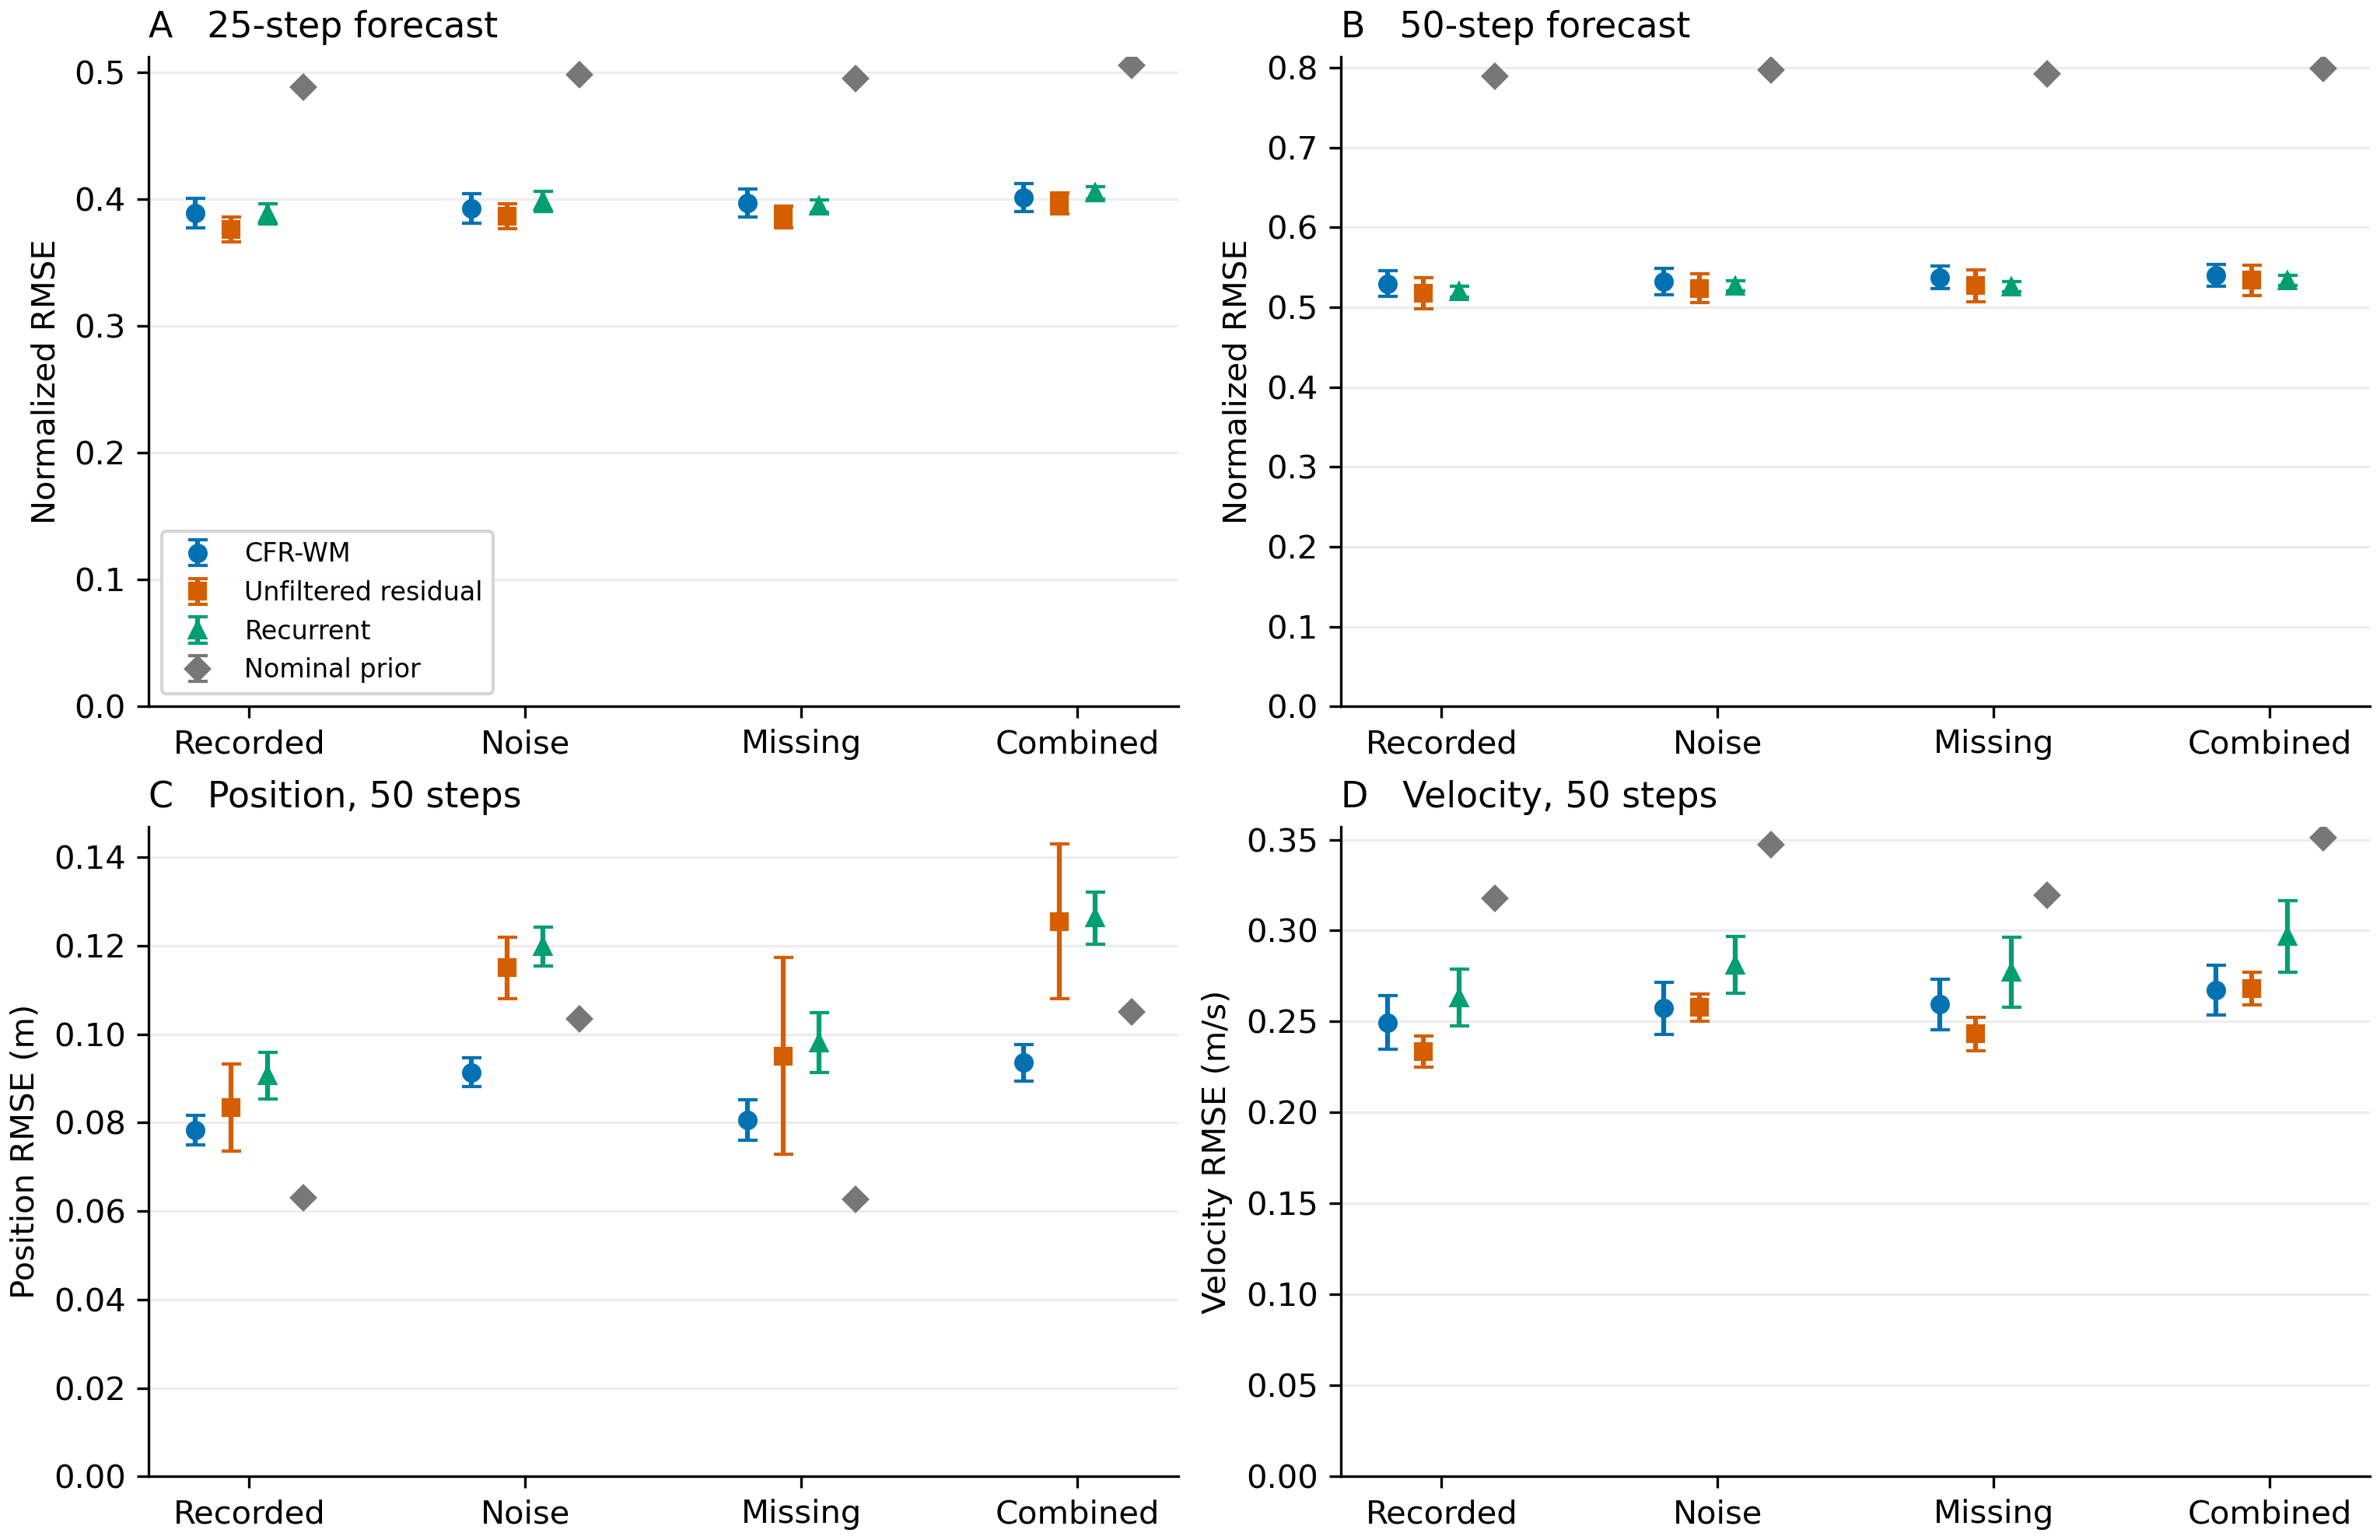
\includegraphics[width=\textwidth]{figures/external_flight.png}
\caption{Prediction on the held-out Melon flights: both normalized-error
horizons and 50-step position and velocity errors. Error bars describe
training-seed variation on the same three test flights.}
\label{fig:external-flight}
\end{figure*}

\section{Discussion}

The frozen analysis \PrimaryInterpretation. The lower bootstrap endpoint
cleared the 5\% practical margin, and the exact seed-level test rejected that
same margin. Together, these results support CFR-WM's aggregate forecasting
advantage across the fixed benchmark, accounting for variation
across eight independent training/data realizations.

The regime decomposition reveals the central trade-off. The
corrupt/shifted estimate was \CorruptImprovement\%, whereas the clean estimate
was \CleanImprovement\%; after hierarchical gating, the full analysis
\RobustnessInterpretation. Context corruption and parameter shift stress
different terms in the error recursion. Noise affects the measurement error in
Equation~\eqref{eq:filter-mse}, while missingness switches off the measurement
correction. Parameter shift biases
the nominal pre-update error and the subsequent nominal rollout. A gain of 0.5
applies the same weighting in these cases. The three cells with more than 10\%
degradation were all clean, led by cart--pole, while every ID-corrupt cell improved
descriptively. This pattern is consistent with noise suppression under
corrupted context and over-correction of already accurate clean context.
The external flight experiment complements this bundled-regime comparison
with separately varied noise and missingness.

The measured flights sharpen this interpretation. The matched unfiltered
model has lower full-state NRMSE in every external condition--horizon mean,
while CFR-WM has lower 50-step position error in all four conditions.
On recorded contexts, its velocity error rises from
\ExternalUnfilteredRecordedLongVelocityMean{} to
\ExternalCFRRecordedLongVelocityMean{}\,m\,s$^{-1}$.
This component dependence is compatible with the conditional error identity:
the same gain acts on channels with different observation errors and
physical-model mismatch. The authors' offline smoothing also changes the
context error relative to raw sensing. Determining which of these factors
causes the observed pattern requires channel-specific interventions.

The gain sweep places equal trust within a continuum of context updates. The
descriptively lowest aggregate NRMSE among the five frozen gains occurred at
\BestGain. The endpoints are pure nominal context propagation (gain 0) and
direct measurement replacement (gain 1). Their relative accuracy depends on
observation noise, nominal-model error, and missingness, which vary by channel
and trajectory. A learned gain was screened during development; its advantage
over the matched fixed-gain model fell below the prespecified mechanism
threshold.

Multi-step training addresses a different part of the recursion. CFR-WM's
relative effect against the one-step-trained variant was
\OneStepImprovement\% (95\% CI [\OneStepRelativeCILow\%,
\OneStepRelativeCIHigh\%]). The context filter changes the initial-error term,
whereas multi-step likelihood exposes the residual transition to its own
forecast distribution and targets accumulated local errors. Their roles are
therefore complementary in the error bound. The paired sensitivity contrast
supports lower error with multi-step training on this benchmark
(Holm $p=\OneStepHolmP$).

The design separates context correction and transition learning through a
measurement rule, explicit missing-channel semantics, known-control free
rollout, and approximately parameter-matched gain comparisons. The clean--corrupted
and position--velocity trade-offs motivate context updates that account for
channel-specific measurement reliability and nominal dynamics. Further extensions
include structured occlusion, ensembles or conformal calibration, and
closed-loop planning
\cite{portela2025_conformal_prediction_for_uncertainty_quantification,brunke2022_safe_learning_in_robotics_from}.

\section{Limitations}

The evidence covers five analytically specified controlled systems and recorded
flights from one drone platform. Both evaluations predict explicit state
coordinates under known future inputs. The external test expands the state
dimension and trajectory family, while additional platforms, visual state
inference, contacts, and closed-loop control remain to be evaluated. NanoDrone
targets are recorded state estimates after offline preprocessing; online sensing
performance requires a separate acquisition and control experiment.

The controlled benchmark uses the correct differential-equation families with
imperfect parameters; the flight prior additionally omits angular acceleration,
drag, and motor lag. Hidden state variables and informative sensor dropout may
change the balance between propagation and correction. Gain 0.5 is fixed;
the gain sweep measures its sensitivity on the controlled benchmark. The
diagonal Gaussian forecast cannot represent multimodality or full cross-state
covariance, and the bounded one-step residual does not guarantee stable
multi-step trajectories.

The synthetic corrupt regimes bundle noise and missingness, with parameter
shift additionally present in OOD-corrupt. The external factorial conditions
separate noise and missingness on released flight records; they leave physical
parameter shift and state-dependent dropout untested. Perturbations model
independent coordinate corruption, whose structure differs from camera
occlusion, sensor outages, or synchronized packet loss.

Controlled-benchmark inference uses eight independent seed-level training/data
realizations. The exact sign-flip test is attainable for the prespecified
five-comparison families, but it has coarse resolution and assumes symmetry of
seed effects. Trajectory resampling improves precision for the fixed benchmark
without creating additional independent training replicates. System--regime
contrasts are consequently descriptive, and inference conditions on the frozen
five-system grid. The external study reports descriptive effects over three
flights from a single platform and collection session. Its five training seeds
quantify optimization variation on those flights; additional acquisition
sessions and platforms are needed to estimate population-level transfer.

\section{Conclusion}

We introduced CFR-WM, a compact world model that combines a prespecified,
mask-exact complementary context update with a probabilistic
physics-residual transition. The design isolates two sources of long-horizon
error: uncertainty in the state at the forecast origin and error accumulated by
the free-rollout transition. A conditional error identity explains when the
fixed update can help, while gain and training-horizon sensitivities evaluate
its contribution to forecast accuracy.

The confirmatory study trained \ConfirmatoryRuns{} models across five
controlled nonlinear systems and three evaluation regimes. Against
the preselected PGNN-style baseline, the seed-balanced relative NRMSE-25 effect was
\PrimaryImprovement\% (95\% CI [\PrimaryRelativeCILow\%,
\PrimaryRelativeCIHigh\%]); accordingly, H1 was \PrimaryDecision, but the
prespecified H2 robustness claim was \RobustnessDecision{} because clean
noninferiority failed. The corrupt/shifted improvement and clean-regime
degradation expose the trade-off introduced by a nonadaptive equal-trust
update.

The measured-flight extension tests a held-out trajectory family with a
structurally simplified physical prior. CFR-WM has higher mean full-state NRMSE
than the matched unfiltered residual model in all eight condition--horizon
comparisons, although its 50-step position error is lower across the four
context conditions. The controlled-benchmark advantage therefore does not
extend to the full-state flight score. These results identify a practical
design trade-off: a fixed context correction can benefit one state component
while worsening the joint forecast. Channel-dependent updates informed by
measurement reliability and physical-model error are a natural next step.

\backmatter

\section*{Declarations}

\textbf{Funding} [To be completed by the authors before submission.]

\textbf{Competing interests} [To be confirmed by the authors before submission.]

\textbf{Ethics approval and consent to participate} The study uses simulated dynamics and publicly released quadrotor flight records. [Authors to confirm the applicable ethics statement before submission.]

\textbf{Consent for publication} Not applicable.

\textbf{Data and code availability} The controlled-system trajectories are generated by the supplied differential-equation code. External evaluation uses the NanoDrone authors' publicly released, offline-preprocessed flight state estimates~\cite{busetto2026_nanodrone}. The accompanying research package contains source code, seeds, split identifiers, checkpoints, saved predictions, metrics, analysis scripts, and data-download URLs with SHA-256 hashes. Upstream flight records are obtained from the authors' repository; this package grants no additional license to those records. [A public archival repository and persistent identifier must be added before submission.]

\textbf{Author contributions} [To be completed by the authors before submission.]

\textbf{Generative-AI assistance} Generative-AI tools assisted drafting and software development. [Human author review and approval of the equations, sources, code outputs, statistical results, and claims remain to be documented. The authors must confirm this disclosure against the selected journal's policy before submission.]

\begin{appendices}
% Keep Hyperref destinations unique when the Springer class resets appendix counters.
\renewcommand{\theHtable}{appendix.\arabic{table}}
\renewcommand{\theHfigure}{appendix.\arabic{figure}}
\renewcommand{\theHequation}{appendix.\arabic{equation}}
\section{Benchmark specification}

Table~\ref{tab:systems} records the simulator time step and nominal
parameterization; Table~\ref{tab:parameter-ranges} gives every sampled training
and OOD interval. All OOD intervals are non-overlapping on every named shifted
parameter. These ranges define the fixed benchmark.

\begin{table*}[ht]
\centering
\caption{Controlled-system definitions. $u$ is scalar in every system.}
\label{tab:systems}
\resizebox{\textwidth}{!}{%
\begin{tabular}{llll}
\toprule
System & State & $\Delta t$ & Nominal parameters \\
\midrule
Damped oscillator & $(q,\dot q)$ & 0.050 & $m=1.0,\; k=1.6,\; c=0.18$ \\
Forced Duffing & $(q,\dot q)$ & 0.040 & $\alpha=-1.0,\;\beta=1.0,\;c=0.25$ \\
Controlled Van der Pol & $(q,\dot q)$ & 0.035 & $\mu=1.2,\;g_u=1.0$ \\
Torque pendulum & $(\sin\theta,\cos\theta,\dot\theta)$ & 0.040 & $g=9.81,\;l=1.0,\;m=1.0,\;c=0.12$ \\
Cart--pole & $(x,\dot x,\theta,\dot\theta)$ & 0.025 & $g=9.81,\;m_c=1.0,\;m_p=0.1,\;l/2=0.5,\;c=0.04$ \\
\bottomrule
\end{tabular}}
\end{table*}

\begin{table*}[ht]
\centering
\scriptsize
\caption{Complete independently sampled physical-parameter intervals. Symbols
follow Table~\ref{tab:systems}; $g_u$ is the Van der Pol control gain.}
\label{tab:parameter-ranges}
\resizebox{\textwidth}{!}{%
\begin{tabular}{lll}
\toprule
System & Training interval & OOD interval \\
\midrule
Damped oscillator & $m\in[0.90,1.10],\ k\in[1.40,1.80],\ c\in[0.14,0.22]$ & $m\in[1.25,1.45],\ k\in[2.05,2.35],\ c\in[0.26,0.34]$ \\
Forced Duffing & $\alpha\in[-1.10,-0.90],\ \beta\in[0.90,1.10],\ c\in[0.20,0.30]$ & $\alpha\in[-0.75,-0.60],\ \beta\in[1.25,1.45],\ c\in[0.34,0.44]$ \\
Controlled Van der Pol & $\mu\in[1.00,1.40],\ g_u\in[0.90,1.10]$ & $\mu\in[1.65,1.95],\ g_u\in[1.25,1.45]$ \\
Torque pendulum & $g\in[9.65,9.95],\ l\in[0.90,1.10],\ m\in[0.90,1.10],\ c\in[0.08,0.16]$ & $g\in[10.25,10.55],\ l\in[1.25,1.45],\ m\in[1.25,1.45],\ c\in[0.20,0.28]$ \\
Cart--pole & $g\in[9.65,9.95],\ m_c\in[0.90,1.10],\ m_p\in[0.085,0.115],\ l/2\in[0.45,0.55],\ c\in[0.02,0.06]$ & $g\in[10.25,10.55],\ m_c\in[1.25,1.45],\ m_p\in[0.135,0.160],\ l/2\in[0.65,0.78],\ c\in[0.075,0.105]$ \\
\bottomrule
\end{tabular}}
\end{table*}

The action generator is a bounded first-order filtered process. At step $t$, a Gaussian innovation with scale $0.55$ times the system action limit is combined with the previous action using coefficients 0.18 and 0.82, then clipped. Limits are 1.5, 1.8, 1.2, 2.2, and 8.0 for the systems in Table~\ref{tab:systems}. This produces persistent excitation independently of the simulated state and defines the control-input distribution.

Train/validation/test separation occurs before window construction. A root NumPy \texttt{SeedSequence} spawns distinct split generators, which in turn spawn one generator per trajectory. The OOD test has a separate root seed. Observation corruption uses another recorded seed after state generation. Consequently, changing an observation-noise level does not change the underlying clean ID trajectory, and all methods see exactly the same corruption draw within a condition.

\section{Candidate selection and confirmatory grid}

Two earlier candidates were screened before the present confirmation. The first, RGP-WM, was rejected after correcting an inappropriate trajectory-local normalization in the development analysis. The second, a learned-gain PFR-WM, was rejected by its frozen selection rule because its NRMSE-25 improvement over the prespecified gain-0.5 sensitivity was 0.223\%, below the required 2\%. Neither candidate appears in the confirmatory grid. The fixed gain of 0.5 used by CFR-WM was selected from that prespecified development sensitivity before any confirmatory seed was generated. Development outcomes are archived separately from the confirmatory analysis.

The immutable grid comprises 11 methods, eight seeds (41, 53, 67, 79, 83, 97, 109, and 113), five systems, and three test regimes. It therefore contains 440 fitted models, 1,320 aggregate evaluation cells, and 126,720 trajectory-level rows. Each seed--system dataset contains 256 training, 64 validation, and 96 test trajectories of 72 time steps. Models receive eight context steps and predict 25 steps open loop. Training observations use noise equal to 3\% of the fixed training-state scale and a nominal 10\% independent missing probability; the corrupt regimes use 8\% observation noise and a nominal 25\% probability. The first time point of each generated trajectory is forced observed in every channel, with independent masks sampled at all subsequent trajectory times; a later sliding-window context can begin with an imputed value. ID-clean and ID-corrupt evaluations share trajectory identifiers; the OOD trajectory set is disjoint.

The five broad comparators are compact, protocol-matched RSSM-style,
SimNorm-style, Transformer-style, PGNN-style, and PG-DMM-style transitions. Five
prespecified CFR sensitivities test gains $0$, $0.25$, $0.75$, and $1$, plus a
one-step-trained gain-0.5 model. CFR-WM retains the unused learned-gain-head
parameters to maintain identical parameter counts across fixed-gain comparisons.

All methods ingest normalized context values, masks, log-one-plus elapsed times,
and actions. Except for the Transformer-style encoder, context is encoded by a
GRU; open-loop recurrent updates use a GRUCell. Every MLP has two hidden linear
layers with SiLU activation. Table~\ref{tab:architectures} lists the remaining
architecture-specific choices.

\begin{table*}[ht]
\centering
\scriptsize
\caption{Exact compact transition architectures used in the confirmatory grid.
The bounded correction is $0.25\tanh(\cdot)$ and all forecast covariances are
diagonal.}
\label{tab:architectures}
\resizebox{\textwidth}{!}{%
\begin{tabular}{llll}
\toprule
Method & Width & Context representation & Forecast transition and variance \\
\midrule
RSSM-style & 80 & GRU; sigmoid feature scaling & data-only MLP mean/log-variance; GRUCell rollout \\
SimNorm-style & 80 & GRU; eight-group simplex projection & data-only MLP mean/log-variance; GRUCell rollout \\
Transformer-style & 48 & two causal layers, four heads, FF width 96, GELU, dropout 0 & data-only MLP mean/log-variance; GRUCell rollout \\
PGNN-style & 84 & GRU & nominal one-substep RK4 plus deterministic residual MLP; learned constant log-variance \\
PG-DMM-style & 84 & GRU & nominal one-substep RK4 plus residual mean/log-variance MLP \\
CFR-WM and gain sensitivities & 72 & GRU states plus mask-exact fixed-gain context update & nominal one-substep RK4 plus residual mean/log-variance MLP \\
\bottomrule
\end{tabular}}
\end{table*}

For CFR-WM, observed context channels use gain 0.5 and missing channels use
gain 0 exactly. The learned gain head remains instantiated but is inactive.
The four gain sensitivities change only the observed-channel gain; the
one-step sensitivity changes only the likelihood horizon.

\section{Frozen hyperparameter search}

The same six learning-rate/weight-decay trials were run on development seed 11
for every system--baseline pair (Table~\ref{tab:tuning-grid}). The stored
reliability-loss weight is shown because it is part of the generic training
configuration, but it is inactive for all confirmatory methods in this paper.
Each baseline uses the validation-NLL winner in
Table~\ref{tab:tuning-winners}; CFR-WM and all CFR sensitivities inherit the
PGNN-style winner for the same system.

\begin{table}[ht]
\centering
\caption{Six-trial frozen optimization grid.}
\label{tab:tuning-grid}
\begin{tabular}{rrrr}
\toprule
Trial & Learning rate & Weight decay & Stored $\lambda_{\mathrm{rel}}$ \\
\midrule
0 & $3\times10^{-4}$ & $10^{-6}$ & 0.1 \\
1 & $6\times10^{-4}$ & $10^{-5}$ & 0.2 \\
2 & $10^{-3}$ & $10^{-5}$ & 0.2 \\
3 & $1.5\times10^{-3}$ & $10^{-4}$ & 0.3 \\
4 & $2\times10^{-3}$ & $10^{-5}$ & 0.4 \\
5 & $3\times10^{-3}$ & $10^{-4}$ & 0.2 \\
\bottomrule
\end{tabular}
\end{table}

\begin{table*}[ht]
\centering
\caption{Frozen winning trial index by system and protocol-matched baseline.}
\label{tab:tuning-winners}
\resizebox{\textwidth}{!}{%
\begin{tabular}{lrrrrr}
\toprule
System & RSSM-style & SimNorm-style & Transformer-style & PGNN-style & PG-DMM-style \\
\midrule
Damped oscillator & 3 & 2 & 4 & 5 & 1 \\
Forced Duffing & 5 & 4 & 5 & 5 & 5 \\
Controlled Van der Pol & 5 & 5 & 5 & 5 & 0 \\
Torque pendulum & 5 & 5 & 5 & 5 & 4 \\
Cart--pole & 5 & 5 & 5 & 5 & 5 \\
\bottomrule
\end{tabular}
}
\end{table*}

\section{Confirmatory estimands and decisions}

H1 is the sole confirmation gate. It asks whether CFR-WM improves fixed-training-scale NRMSE-25 over the preselected PGNN-style comparator by at least 5\%. Within each seed, PGNN-style and CFR-WM are averaged with equal weight over all 15 fixed system--regime cells; the primary point estimate is the arithmetic mean of the eight seed-specific relative improvements. H1 requires finite metrics, a 95\% bootstrap lower endpoint of at least 5\%, and a one-sided exact sign-flip $p<0.05$ for the 5\% margin.

H2 is a hierarchically gated robustness claim. Conditional on H1, the combined corrupt and parameter-shifted regimes must satisfy the same 5\% improvement rule, while ID-clean performance must be noninferior under a signed relative margin of $-5\%$. Both components require their corresponding bootstrap lower endpoint to meet or exceed the margin and a one-sided exact sign-flip $p<0.05$. If H1 fails, H2 is not supported irrespective of its component estimates.

The bootstrap uses 5,000 replicates. Each replicate resamples the eight seed clusters globally with replacement and then resamples paired trajectory identifiers within every retained seed--system block. A single sampled identifier vector is reused for ID-clean and ID-corrupt repeated measurements, whereas the disjoint OOD identifiers are sampled separately. All five systems and three regimes remain in every replicate, and baseline, candidate, and their relative ratio are recomputed within the replicate. Exact tests enumerate all $2^8$ seed-level sign flips and therefore rely on a seed-effect symmetry assumption. The five broad-comparator contrasts and the five sensitivity contrasts form separate Holm-adjusted families. The 15 system--regime contrasts are descriptive and carry no cell-level significance claim.

\section{Provenance and analysis amendment}

The frozen contract records the method list, seeds, data design, training configuration, success rules, and SHA-256 hashes of the training, evaluation, analysis, and tuning artifacts. The dedicated runner rejects command-line overrides and resumes only provenance-matched JSON/checkpoint pairs. The generic development runner rejects every frozen seed and the reserved confirmatory output directory. Analysis aborts unless the exact grid, finite metrics, trajectory pairing, disjoint OOD identifiers, 40 distinct seed--system data hashes, and stored provenance all validate.

The first frozen-analysis invocation failed before inferential resampling and wrote no result directory because the generic loader had not copied the existing top-level \texttt{parameter\_count} metadata into the aggregate frame used for descriptive model-size reporting. The archived amendment was frozen before performance inspection. It adds only that field by a method--seed--system many-to-one join, verifies all 440 JSON/checkpoint pairs and the completed-run manifest, and then invokes the unchanged frozen inference functions. The failed log, original analysis hash, amendment code hash, and amendment-contract hash are included in the reproduction package. No trajectory metric, hypothesis, threshold, resampling seed, replicate count, multiplicity family, or decision changed.

The top-level independent units are the eight stochastic training/data realizations, with trajectories nested within them. Statistical inference concerns the prespecified finite benchmark and variation across the frozen seed realizations.

\section{Complete descriptive cell contrasts}

Table~\ref{tab:all-cell-contrasts} reports every prespecified CFR-WM--PGNN-style
system--regime contrast. Absolute intervals come from the paired nested
bootstrap. Relative changes use PGNN-style as the denominator, with negative values
favoring CFR-WM. These fixed-cell estimates are descriptive.

\begin{table*}[ht]
\centering
\small
\caption{All 15 descriptive CFR-WM versus PGNN-style NRMSE-25 contrasts.}
\label{tab:all-cell-contrasts}
\resizebox{\textwidth}{!}{\begin{tabular}{llrr}
\toprule
System & Regime & CFR--PGNN-style [95\% CI] & Relative change, \% \\
\midrule
Cartpole & ID clean & +0.0163 [+0.0103, +0.0225] & +47.33 \\
Cartpole & ID corrupt & -0.0207 [-0.0281, -0.0136] & -13.33 \\
Cartpole & OOD + corrupt & -0.0111 [-0.0194, -0.0027] & -5.66 \\
Controlled Van Der Pol & ID clean & +0.0059 [-0.0022, +0.0149] & +19.36 \\
Controlled Van Der Pol & ID corrupt & -0.0318 [-0.0381, -0.0250] & -32.39 \\
Controlled Van Der Pol & OOD + corrupt & -0.0083 [-0.0148, -0.0016] & -4.74 \\
Damped Oscillator & ID clean & -0.0011 [-0.0041, +0.0019] & -2.41 \\
Damped Oscillator & ID corrupt & -0.0291 [-0.0341, -0.0244] & -32.12 \\
Damped Oscillator & OOD + corrupt & -0.0257 [-0.0295, -0.0223] & -27.86 \\
Forced Duffing & ID clean & +0.0094 [+0.0028, +0.0168] & +24.37 \\
Forced Duffing & ID corrupt & -0.0295 [-0.0342, -0.0249] & -30.24 \\
Forced Duffing & OOD + corrupt & +0.0094 [+0.0011, +0.0174] & +3.90 \\
Torque Pendulum & ID clean & -0.0046 [-0.0082, -0.0005] & -8.59 \\
Torque Pendulum & ID corrupt & -0.0378 [-0.0436, -0.0316] & -34.80 \\
Torque Pendulum & OOD + corrupt & +0.0110 [+0.0055, +0.0165] & +5.94 \\
\bottomrule
\end{tabular}
}
\end{table*}
\end{appendices}

\bibliography{../references,../external_references}
\end{document}
